\documentclass[english,version-2020-11]{uzl-thesis}
\usepackage{placeins}

% Copy this file as a template for your thesis. You will have to take
% action at all places marked by
%
% !!!!!!!!!!!!!!!!!!!!!!!!!!!!!!!!!!
% !!! Your action is needed here !!!
% !!!!!!!!!!!!!!!!!!!!!!!!!!!!!!!!!!
%
% The first place your action is needed is the first line of this
% document:
%
%
% Language of the thesis:
%
% You must use either 'german' or 'english' above, depending on the
% language used in the main text. This will automatically setup a lot
% of things in the background.
%
%
% Version of the class:
%
% You must specify which version of the thesis class is to be
% used. This is important in case the class style changes in later
% years, but we still want an older thesis to look the same, even when
% things are changed in the class.
%
% Do not change or remove the version-xxxx key.
%
%
% Text encoding:
%
% Your thesis *must* be encoded in utf8 (unicode), which is the
% default in most editors these days. Do *not* change this to latin8.



%%%
%
% Main setup:
%
%%%
%
% You must use the \UzLThesisSetup command to specify numerous things
% about your thesis. This includes the entries on the title page, the 
% abstracts, and the bibliography style. You do so by specifying
% so-called "values" for so-called "keys". For instance, 
% for the key "Autor" you must provide your name as the value. You do
% so by writing 'Autor = {Max Mustermann}', that is, the value is put
% into curly braces. You can use the \UzLThesisSetup command
% repeatedly and the order in which you provide the keys is not
% important. 
%
% Everything shown on the title page must be in German -- even
% if the thesis is written in English! Just insert German text for
% German keys and English text for English keys (like 'Abstract' needs
% English text, while 'Zusammenfassung' needs German text).

\UzLThesisSetup{
  %
  % !!!!!!!!!!!!!!!!!!!!!!!!!!!!!!!!!!
  % !!! Your action is needed here !!!
  % !!!!!!!!!!!!!!!!!!!!!!!!!!!!!!!!!!
  %
  % First, specify the institut or clinic at which the thesis was
  % written. You get the logo file from them (make sure it has the
  % correct size, namely the same as the example). If they do not have
  % a logo, the university's default logo is used.
  %
  % The 'verfasst' gets two arguments. Change the first to {an der}
  % for clinics, as in 'Verfasst = {an der}{Medizinischen Klinik I}'
  %
  Logo-Dateiname        = {uzl-thesis-logo-uzl.pdf},
  Verfasst              = {am}{Institut für Software Engineering und Programming Languages},
  %
  % The titles:
  %
  Titel auf Deutsch     = {
    Können semantische Ähnlichkeiten von Wörtern die Schlussfolgerungen des gesunden Menschenverstands verbessern?  Eine Fallstudie mit Prover E und SUMO.
  }, 
  Titel auf Englisch    = {
    Can semantic similarities of words enhance common sense reasoning?  A case study with prover E and SUMO.
  },
  %
  % Author and supervisor:
  % 
  % Note that the 'Betreuer' or 'Betreuerin' is the supervisor, that
  % is, the professor who officially supervises the thesis. If there
  % is also an assistent of the professor who helped (typically a
  % lot), use 'Mit Unterstützung von' to thank that person. If the
  % thesis was mainly written 'externally' at some company or another
  % institute, point this out using 'Weitere Unterstützung'. 
  % 
  % For your own name, do *not* add things like "BSc" or "BSc
  % cand.". For the supervisor, you should normally include
  % "Prof. Dr." or "PD Dr." (ask your supervisor, what is
  % appropriate), but nothing more (so no
  % "Univ.-Prof. Dr. Dr. h.c. mult." unless your supervisor insists).  
  %
  Autor                 = {Julian Britz},
  Betreuerin            = {Prof. Dr. Diedrich Wolter},
  % 
  % Optional: Supporting persons and institutions. The text should be
  % in German, even for an English thesis.
  %
  Mit Unterstützung von = {Moritz Bayerkuhnlein},
  % 
  %   Weitere Unterstützung = {
  %     Die Arbeit ist im Rahmen einer Tätigkeit bei der Firma Muster GmbH
  %     entstanden.
  %   },
  %
  %
  % Your Degree Programm (Studiengang)
  %
  % Specify 'Bachelorarbeit' or 'Masterarbeit' and the degree
  % programme. Make sure the name of programme is correct and not
  % some abbreviation or some incorrect variant. For instance:
  % 'Medizinische Ingenierwissenschaft', but not 'MIW';
  % 'Medizinische Informatik', but not 'Medizin-Informatik';
  % 'Informatik', but not 'Informatik (SSE)'.
  %
  % Use German names for German programmes and English names for
  % English ones, so 'Infection Biology', not 'Infektionsbiologie'. 
  % For programmes that have a German bachelor and an English master,
  % use the German name for a bachelor thesis and the English name for
  % the master thesis.
  %
  Bachelorarbeit,
  Studiengang           = {Informatik},
  %
  % Date on which the thesis is turned in German, formatted the
  % traditional German way:
  %
  Datum                 = {06. Juli 2025},
  %
  % The English abstract. You must always provide abstracts in German
  % and in English. 
  %
  Abstract              = {
    Abstract
  },
  Zusammenfassung       = {
    Zusammenfassung 
  },
  %
  % Optional: 'Danksagungen' (German) or 'Acknowledgements'
  % (English). Both keys are optional and both have the same effect of
  % adding an acknowledgements text after the abstracts and before the
  % table of contents.
  %
  Acknowledgements      = {
    Acknowledgements
  },
  % Bibliography style: Choose between
  % 
  % 'Alphabetische Bibliographie'
  % for all degree programmes in the natural sciences 
  % 
  % 'Numerische Bibliographie'
  % alternative for all other degree programmes
  % 
  % Either will load biblatex and setup the citation methods and the
  % bibliography styles correctly. You should not mess with them.
  % 
    Alphabetische Bibliographie,
  % Alternatively:
  % Numerische Bibliographie
}




%%%%%%%%%%%%%%%%%%%%
%
% Styling the thesis
%
%%%%%%%%%%%%%%%%%%%%
%
% Creating a visually pleasing layout and choosing fonts is not
% easy. Furthermore, different people have different preferences. Of
% course, for the University of Lübeck, the dean of studies could just
% force everyone to use one specific layout and font, but that seems a
% bit drastic and, also, it seems nice that thesis by different people
% have an individual style even though they all stick to the same
% overall structure.
%
% For these reasons, I (Till Tantau) have spend quite some time on
% designing a flexible layout and styling mechanism for theses.
%
% Basically, the overall structure of the thesis is fixed by the
% thesis class and so are many structural elements. For instance, you
% cannot change the order in which the abstract and table of contents
% are shown, you cannot move the bibliography elsewhere, indeed, the
% bibliography style is also fixed. Likewise, the text on the title
% page is fixed.
%
% Although many things are fixed, you *can* change several other
% things. For instance, you can change the font used for the main
% text, you can change which font is used for titles and headings or
% you can change whether titles and headlines are centered or flushed
% left.
%
% There are many LaTeX packages for changing such things. You are
% kindly asked *not to use them*. Rather, use (only) the options
% offered by the thesis class. All possible choices and combinations
% there have been tested by me and produce nice results; what happens
% with other packages no one knows and might no longer conform to what
% is expected by the university. As you will see, you still have a
% lot of options.
%
%
% Technical note: All styling is done via the command
%
% \UzLStyle{...}
%
% where ... is a key-value list just as for \UzLThesisSetup. The
% difference is just that everything having to do with styling as
% controlled by \UzLStyle, while the more “formal” setup keys are
% controlled by \UzLThesisSetup.
%
%%%
%
% Designs
%
%
% A \emph{design} is a whole set of font and layout options bundled
% together. They have been chosen in such a way that a visually
% pleasing “overall appearance” results.
%
%
% \UzLStyle{computer modern oldschool design}
%
% The look of this design mimics the “classical” way a paper or report
% created with \LaTeX\ looks like: The Computer Modern font is used,
% bold face fonts are used for headlines, only black and white are
% used as colors. This design reminds me of older scientific
% documents, especially from the computer science community where
% \LaTeX\ was used very early.
%
%
% \UzLStyle{computer modern basic design}
%
% A slightly less “oldschool” version of the previous design. It is
% still a classic design in the sense that it uses the Computer Modern
% font and that it still has this “good old \LaTeX” look, but some
% more modern aspects (like colors!) have been added.
%
% Note that this design uses Myriad for the title page (one of the
% “modern aspect”), which means that his font must be installed.
%
%
% \UzLStyle{computer modern scholary design}
%
% In my opinion, this is the ultimate “scholary design”: The thesis
% will look like it has been typeset by hand some 150 years ago and
% then printed by a university press. There is really nothing “modern”
% about it and the word in the name of the design is just part of the
% name of the “Computer Modern” font.
%
%
% \UzLStyle{pagella basic design}
%
% A, well, basic design that uses the Pagella font rather than the
% Computer Modern font. Especially the bold face version of this font
% looks nicer than the Computer Modern counterpart. Also, Pagella,
% while still having a “bookish” look, still feels a bit fresher than
% Computer Modern. 
%
%
% \UzLStyle{pagella centered design}
%
% A variant of the basic Pagella design that centers all
% headlines. A nice alternative to the basic version.
%
%
% \UzLStyle{pagella contrast design}
%
% This design tries to create some visual friction by contrasting the
% sans serif headline font (in bold!) with the main text. I find it a
% visually very interesting combination.
%
%
% \UzLStyle{alegrya basic design}
%
% The third variant of the basic design, this time using the Alegrya
% font. 
%
%
% \UzLStyle{alegrya scholary design}
%
% The Alegrya version of the previous “scholary” design. Unlike the
% Computer Modern version, this design does not look old, but more
% fresh -- while still creating the impression that the text must be
% about a very scientific subject. 
%
%
% \UzLStyle{alegrya stylish design}
%
% The design is quite similar to the scholary version for the Alegrya
% font, but with even more modern additions. “Stylish” is the word
% that comes to my mind.
%
%
\UzLStyle{alegrya modern design}
%
% A design that uses the sans serif version of the Alegrya font for
% the headlines. This is a nice modern overall design.
%
%%%




%%%%%%%%
%
% Now, include the package you need here using \usepackage. 
%
% However, many standard packages are already loaded by the class:
%
% amsmath, amssymb, amsthm, babel, biblatex, csquotes, etoolbox,
% filecontents, fontspec, geometry, hyperref, tikz (with libraries
% arrows.meta, positioning and shapes), varioref, url 
%
% Indeed, in many cases you will not need any extra packages.
%
%%%%%%%





\begin{document}

%
% The title page and table of contents will be inserted automatically
% here. 
%


\chapter{Introduction}
\label{chapter-introduction}

Automated theorem proving is a fundamental technique in formal logic and artificial intelligence. 
It enables the validation of logical statements based on a given set of axioms and inference rules. 
This thesis investigates whether incorporating frequently used axioms, referred to as core axioms, into a subset of the Adimen SUMO grammar improves proof success rates. 
The selected subset is determined by combining syntactic and semantic criteria to ensure both structural and conceptual relevance.

\section{Problem Statement}
Given a formal logical grammar, such as Adimen SUMO, and a conjecture \( C \), the objective is to identify a subset of axioms that maximizes the probability of proving \( C \). The process involves:
\begin{itemize}
    \item Selecting axioms based on syntactic and semantic similarity, forming a set denoted as \( \mathcal{A}_{\text{rel}} \).
    \item Testing whether adding frequently used axioms, \( \mathcal{A}_{\text{core}} \), improves proof success.
\end{itemize}

Even though there is no direct mapping between natural and logical language, we assume, that there is an entanglement between them: \\
\begin{equation}
    \mathcal{L}_{\text{NL}} \bowtie \mathcal{L}_{\text{logic}}
\end{equation}

Arguments for this assertion are that logical langugage is human made and therefore inevitably connected to human and consequently natural language.
Also grammers like Adimen SUMO are partially derived by lexical-semantic networks that capture relationships between words of natural language.
Making use of this entanglement the selection process of theorem proovers can be optimized by reducing the number of relevant axioms.
Theorem prover E follows a refutational proof procedure using the superposition calculus. The proof search is based on a modified given-clause algorithm, consisting of several key steps:

\begin{enumerate}
    \item Initialization: The input problem is converted into clausal normal form (CNF) and divided into two sets: unprocessed clauses \( U \) and processed clauses \( P \).
    \item Clause Selection: A clause \( g \) is selected from \( U \) based on heuristics, referred to as the given clause, and is then simplified against \( P \).
    \item Simplification: The given clause undergoes forward simplification using processed clauses. This step removes redundant literals, applies rewriting rules, and ensures that terms are arranged in a canonical order.
    \item Inference: The prover applies the superposition calculus, combining \( g \) with clauses in \( P \) to generate new clauses. These new clauses are simplified and added to \( U \) if they are neither trivial nor redundant.
    \item Saturation or Termination: The process stops when:
    \begin{itemize}
        \item The empty clause \( \bot \) is derived, confirming the proof.
        \item The clause set is saturated, meaning no further inferences can be made.
        \item A predefined resource limit, such as time or memory, is reached.
    \end{itemize}
\end{enumerate}
\cite{Schulz2019}

Axioms play a crucial role in simplification. While the prover cannot arbitrarily discard axioms, as they form the foundation of logical reasoning, they are essential for clause rewriting and subsumption.


\section{Hypothesis}

To test whether adding frequently used axioms improves proof success, we define the key elements of the problem:

\begin{itemize}
    \item \( \mathcal{A} \) represents the full set of axioms available in Adimen SUMO.
    \item \( C \) is the conjecture we want to prove.
    \item \( d \) is a function that measures how similar an axiom is to the conjecture, based on both syntax and meaning.
    \item \( \mathcal{A}_{\text{rel}} \) is the set of \( k \) axioms that are most similar to the conjecture according to \( d \):
    \begin{equation}
        \mathcal{A}_{\text{rel}} = \{ A \in \mathcal{A} \mid A \text{ is among the } k \text{ closest axioms to } C \text{ w.r.t. } d \}
    \end{equation}
    \item \( \mathcal{A}_{\text{core}} \) is a collection of axioms that have been used frequently in past proofs.
    \item The enhanced axiom set, \( \mathcal{A}_{\text{enh}} \), is created by combining the most similar axioms with the frequently used ones:
    \begin{equation}
        \mathcal{A}_{\text{enh}} = \mathcal{A}_{\text{rel}} \cup \mathcal{A}_{\text{core}}
    \end{equation}
    \item \( P(T, \mathcal{A}', C) \) is a function that checks if the theorem prover \( T \) is able to prove \( C \) using a given set of axioms \( \mathcal{A}' \). If the proof is successful, the function returns true; otherwise, it returns false.
\end{itemize}

The hypothesis we test is:

\begin{equation}
    \forall C \in \mathcal{C}, \quad \Pr(P(T, \mathcal{A}_{\text{enh}}, C) = \text{True}) > \Pr(P(T, \mathcal{A}_{\text{rel}}, C) = \text{True})
\end{equation}

In other words, the likelihood of proving a conjecture is higher when frequently used axioms are included along with the most similar ones.


\section{Justification and Implications}

Adimen SUMO's grammar is closely connected to natural language structures. 
This means that selecting axioms based on semantic embeddings, such as SBERT, helps capture underlying logical dependencies that might not be immediately apparent. Frequently used axioms act as structural anchors within this system, making it easier for the theorem prover to navigate the proof search space and discover relevant inference steps.
By combining the most relevant axioms with those that have been frequently used in past proofs, the theorem prover benefits from both semantic alignment and structural consistency. This increases the overall proof success rate, as the prover has access to axioms that not only appear relevant but have also proven useful in previous reasoning tasks.

This thesis tests this hypothesis through empirical experiments, measuring proof success rates across different axiom selection strategies. The goal is to determine how much incorporating core axioms improves theorem proving performance.


% DELETE the following line for your own thesis - it causes trouble!
\lstMakeShortInline[style=code,style=inline,language={[LaTeX]tex},moretexcs={chapter}]|


% !!!!!!!!!!!!!!!!!!!!!!!!!!!!!!!!!!
% !!! Your action is needed here !!!
% !!!!!!!!!!!!!!!!!!!!!!!!!!!!!!!!!!
%
% Replace with a detailed account of what other people have already
% researched concerning your thesis's theme. Even when (indeed,
% especially when) there has been only little or even no research by
% other people, you should explain in detail that this is the case and
% why it is the case. 


\section{Structure of this Work}

This thesis is structured into several chapters, each addressing different aspects of the research problem and methodology. It begins with an overview of existing research, followed by the theoretical foundations, the proposed approach, experimental evaluations, and concluding discussions.

Chapter \ref{chapter-relatedwork} provides a review of related work. It covers previous research on theorem proving and axiom selection techniques, as well as how semantic similarity has been applied in logical reasoning.

Chapter \ref{chapter-preliminaries} introduces fundamental concepts necessary to understand the core of this research. It discusses topics such as common sense reasoning, word embeddings, and theorem proving. Additionally, it explains the role of formal grammars and axiom selection in automated reasoning.

Chapter \ref{chapter-experiments} focuses on the experimental setup and evaluation. It outlines the benchmark datasets, describes the evaluation metrics, and presents the results of different axiom selection strategies. The impact of incorporating core axioms into theorem proving is analyzed based on empirical findings.

Chapter \ref{chapter-conclusion} summarizes the main contributions of this work and highlights key insights gained from the experiments. It also discusses potential future directions and remaining challenges in axiom selection and automated reasoning.

Finally, Chapter \ref{chapter-futerwork} explores ideas for future research, suggesting possible extensions and refinements to the proposed approach.

Each chapter builds upon the previous ones, providing a structured progression from theoretical background to practical implementation and evaluation.



\chapter{Related Work}
\label{chapter-relatedwork}

A significant part of this thesis builds upon the work of Schon \cite{Schon2024}, which explores context-specific axiom selection using large language models. Traditional axiom selection methods primarily rely on syntactic properties, often ignoring the meaning embedded in symbol names. Schon proposes an alternative approach by leveraging large language models to determine relevant axioms based on contextual similarity. This method aligns axiom selection with the goal’s context, improving performance in commonsense reasoning tasks. Experiments show that this approach outperforms purely syntactic selection methods, demonstrating the potential of semantic similarity for guiding theorem provers.

The findings of Schon's work play a crucial role in this thesis, as a major aspect of the proposed approach involves using semantic embeddings for axiom selection. However, while Schon focuses on direct context-based selection, this thesis investigates the impact of incorporating frequently used axioms into the selection process. The goal is to determine whether combining core axioms with those chosen based on semantic similarity enhances proof success rates.

Beyond Schon’s work, several other studies have contributed to axiom selection and theorem proving. Adimen-SUMO, developed by Álvarez et al. \cite{Alvez2014}, is a reengineered version of the SUMO ontology designed to improve compatibility with first-order theorem provers. The restructuring ensures that axioms are formulated in a way that facilitates inference, reducing ambiguities present in the original SUMO. This ontology serves as a key resource in evaluating theorem provers, including those used in this thesis.

Syntactic axiom selection has also been widely explored. Hoder and Voronkov \cite{Hoder2011} introduced SInE, a system that selects axioms based on their syntactic relevance to the conjecture. By iteratively choosing axioms that introduce symbols appearing in the conjecture, SInE reduces the search space, making large knowledge bases more manageable. Similarly, Roederer et al.

Another relevant contribution comes from Álvarez et al. \cite{Alvez2017}, who introduced a framework for systematic white-box testing of first-order logic ontologies. Their work focuses on ensuring logical consistency and eliminating redundant or contradictory axioms. Automated testing techniques from this study provide insights into ontology refinement, which is relevant when evaluating the quality of selected axioms in theorem proving.

In summary, Schon’s research serves as the primary foundation for this thesis, providing a framework for semantic axiom selection that is further extended through the integration of frequently used axioms. Other related studies on syntactic axiom selection, ontology structuring, and logical consistency contribute valuable insights, supporting the refinement of the proposed approach.


% !!!!!!!!!!!!!!!!!!!!!!!!!!!!!!!!!!
% !!! Your action is needed here !!!
% !!!!!!!!!!!!!!!!!!!!!!!!!!!!!!!!!!
%
% Replace the whole text chapter with the main text of your thesis! 

\chapter{Preliminaries}
\label{chapter-preliminaries}

This chapter introduces fundamental concepts relevant to this work. It covers common sense reasoning, word embeddings, formal grammars, automated theorem proving, and axiom selection strategies. These topics form the theoretical foundation for the experiments and analyses presented in later chapters.

\section{Common Sense Reasoning}

Common sense reasoning is an essential part of human cognition, allowing individuals to understand everyday situations, infer unstated knowledge, and make reasonable decisions even when information is incomplete. Automated reasoning systems attempt to replicate this ability to improve inference and decision-making.

Common sense reasoning involves recognizing unstated premises in logical arguments, understanding cause-effect relationships, and applying heuristics to solve problems under uncertainty. It plays a key role in artificial intelligence, particularly in natural language understanding, where context is crucial for interpreting meaning, and in automated reasoning, where structured logical frameworks help infer conclusions from available premises. Applications in law, medicine, and finance further highlight the importance of integrating knowledge-based reasoning for interpretability and reliability. Despite advancements in AI, deep learning models struggle with incorporating structured and generalizable knowledge, making common sense reasoning an ongoing challenge.

Interpreting a sentence often involves more than just processing its words—it requires incorporating background knowledge to make sense of implicit information. Take, for example, the Winograd Schema involving John and Billy viewing a stage \cite{Levesque2012}. While the sentence itself is simple, understanding it correctly depends on a series of assumptions that humans naturally make when constructing a mental model of the situation \cite{Bayerkuhnlein2023}.

A stage is something meant to be viewed. In a typical setting, viewers remain stationary, and obstructions can block their line of sight. Humans are physical entities, meaning they cannot see through solid objects. Both John and Billy are human names, so the sentence suggests a scene where one person is obstructing the other’s view. The interpretation of who is blocking whom depends on the additional context provided by the sentence, but the reasoning process remains the same: we piece together knowledge about how the world works to arrive at a coherent understanding.

These intuitive assumptions form the foundation of common sense reasoning. The process aligns with the theory of mental models, which suggests that humans construct internal representations of a scenario to evaluate possible interpretations \cite{JohnsonLaird1989}. In the case of ambiguous pronouns, this internal model helps determine which assignment makes the most logical sense. This ability to build structured mental representations is what allows humans to effortlessly resolve ambiguities that challenge AI systems.

\section{Word Embeddings}

Word embeddings represent words as numerical vectors in a continuous space, capturing semantic relationships based on their contextual usage. Unlike traditional representations such as one-hot encoding, embeddings enable words with similar meanings to be positioned closer together in the vector space, allowing models to generalize across linguistic variations. 

Different techniques have been developed to generate word embeddings, each with unique properties and advantages. Word2Vec \cite{Mikolov2013} is one of the foundational models, introducing two architectures: Continuous Bag of Words (CBOW) and Skip-gram. CBOW predicts a word based on its surrounding context, while Skip-gram does the inverse, predicting context words given a target word. This approach efficiently captures both syntactic and semantic relationships. FastText \cite{Bojanowski2017} extends Word2Vec by incorporating subword information, representing words as bags of character n-grams. This allows it to handle rare words and out-of-vocabulary terms better than standard word-based models. GloVe \cite{Pennington2014}, in contrast, constructs embeddings by factorizing a word co-occurrence matrix, capturing both local and global semantic information.

The effectiveness of word embeddings depends on several factors, including the size of the context window, the type of training data, and the inclusion of subword information.

Beyond standard word embeddings, contextual embeddings such as BERT and GPT \cite{Devlin2019} further refine representation by considering the full sentence structure, allowing word meanings to dynamically change based on context. This advancement is particularly relevant in cases where words have multiple meanings depending on their use in different sentences.

In this work, word embeddings are leveraged to determine the semantic similarity between axioms and conjectures. By using pre-trained models like Sentence-BERT (SBERT), it becomes possible to enhance axiom selection in theorem proving, ensuring that the selected axioms are not only structurally relevant but also semantically meaningful.


\section{Grammars in Natural and Formal Languages}

Grammars define the structural rules of a language, whether it is a natural language like English or a formal system used in logic. In theorem proving, grammars are essential for structuring logical statements in a way that machines can interpret and manipulate.

Different types of grammars serve various purposes. Context-free grammars (CFGs) define syntactic structures in natural language processing and programming languages. First-order logic (FOL) grammars represent logical expressions using predicates, functions, and quantifiers. Ontology-based grammars, such as SUMO (Suggested Upper Merged Ontology) \cite{Niles2001}, combine linguistic and logical structures to improve knowledge representation.

Grammars are crucial in theorem proving because they enforce logical consistency, allow automated systems to process logical expressions systematically, and provide a structured representation of knowledge in formal systems like SUMO and Adimen-SUMO.

\section{Automated Theorem Proving}

Automated theorem proving aims to determine whether a given conjecture follows logically from a set of axioms. It is a key component of formal logic and artificial intelligence.

Theorem provers rely on different proof strategies. Logical inference derives new statements from existing ones using formal rules. Resolution is a proof technique that derives contradictions, commonly used in first-order logic provers. Refutation works by attempting to show that a conjecture holds by deriving a contradiction from its negation.

Prover E is a widely used theorem prover based on the superposition calculus \cite{Schulz2013}. It follows a structured process where input formulas are first converted into conjunctive normal form (CNF). The prover then selects clauses heuristically, applies inference rules such as resolution and superposition to generate new clauses, simplifies redundant ones, and continues searching until either an empty clause is derived, proving the conjecture, or computational resources are exhausted. Understanding these mechanisms is important for optimizing axiom selection.

\section{Axiom Selection Strategies}

Theorem provers often struggle with large search spaces, making axiom selection a critical challenge. The process of selecting axioms influences proof efficiency and success rates.

\section{Syntax-Based Selection: SInE}

The SInE selection strategy \cite{Hoder2011} is a trigger-based approach designed to efficiently select axioms in automated theorem proving. Instead of selecting axioms based on fixed rules, it dynamically determines relevance using a trigger relation. This relation ensures that an axiom is only selected if at least one of its symbols appears less frequently than or as frequently as all other symbols in the axiom. This prevents highly common symbols from triggering every axiom they appear in, reducing unnecessary selections.

The selection process starts by identifying symbols that appear in the conjecture to be proven. These symbols are considered directly triggered. If a triggered symbol appears in an axiom and satisfies the trigger relation, the axiom is selected, and its other symbols become triggered in the next selection step. This process continues recursively up to a defined depth \( k \), ensuring that only the most relevant axioms are included.

One limitation of this approach arises when an axiom contains symbols with nearly equal occurrence counts. In such cases, only the least frequent symbol can trigger the axiom, potentially excluding useful axioms. To address this, a benevolence parameter \( b \) is introduced, allowing symbols that occur up to \( b \) times more frequently than the least common symbol to also act as triggers. This adjustment provides more flexibility in axiom selection.

\section{Vector-Based Selection}

Syntax-based selection methods like SInE do not consider the meaning of symbol names, which can lead to the loss of useful information. This is particularly problematic in commonsense reasoning, where symbol names often carry semantic meaning that could improve selection. To address this, vector-based selection methods leverage word embeddings to quantify the semantic similarity between axioms and the goal.

As seen above, word embeddings are a common technique in natural language processing, based on the distributional hypothesis \cite{Miller1991}. This hypothesis states that words appearing in similar contexts tend to have similar meanings. By training neural networks on large text corpora, words are mapped into a continuous vector space, where their geometric relationships capture semantic similarity. Cosine similarity is commonly used to measure the closeness of two word vectors, with values ranging from -1 (completely dissimilar) to 1 (identical).
\\
\textbf{Definition 5.1 (Cosine similarity of two vectors \cite{Schon2023}).}  
Let \( \mathbf{u}, \mathbf{v} \in \mathbb{R}^n \) be non-zero vectors. The cosine similarity of \( \mathbf{u} \) and \( \mathbf{v} \) is defined as:

\[
\text{cos sim}(\mathbf{u}, \mathbf{v}) = \frac{\mathbf{u} \cdot \mathbf{v}}{\|\mathbf{u}\| \|\mathbf{v}\|}
\]
\\

Schon \cite{Schon2023} introduces a statistical approach for axiom selection that relies on word embeddings to represent axioms as vectors. The idea is to encode axioms into a continuous vector space where semantically similar axioms are mapped closer together. This is done in a preprocessing step, where each axiom in the knowledge base is transformed into a vector representation using a word embedding model.

When selecting axioms for a given goal \( G \), the goal is vectorized in the same way as the axioms in the knowledge base. The selection process then identifies the \( n \) axioms whose vector representations are most similar to that of \( G \). The similarity between vectors is measured using cosine similarity, which quantifies how closely two vectors align regardless of their magnitude.

Formally, given a knowledge base \( KB \), a goal \( G \), and a vectorization function \( f \) that maps axioms to \( \mathbb{R}^n \), the vector-based selection process selects the \( n \) axioms in \( KB \) that have the highest cosine similarity to \( G \). The selected axioms form a subset of \( KB \) where no other axiom outside this subset has a higher similarity to \( G \) than the least similar axiom within the selected set.

This approach ensures that axioms most relevant to the goal, based on their semantic similarity, are prioritized during the selection process.

\section{SeVEn: Sentence-Based Vector Encoding}

Sentence embeddings function similarly to word embeddings, as they are also generated by training neural networks on large text corpora. However, while word embeddings focus on individual words, sentence embeddings capture the meaning of entire sentences or even full documents \cite{Kiros2015SkipThought}. This ability makes them particularly useful for encoding more complex relationships between axioms.

Following this idea, the SeVEn approach builds upon vector-based selection by modifying how axioms are represented. Instead of encoding individual symbol names, each axiom is first translated into a sentence that captures its semantic meaning. This sentence is then encoded into a vector using a sentence embedding model. The overall process remains similar to standard vector-based selection, but the vectorization method is adapted to work at the sentence level. Given a knowledge base \( KB \), where each axiom \( A \) is transformed into a sentence \( S \) using a function \( t \), the sentence embedding function \( f \) then maps \( S \) into a vector representation \( v_S(A) \). The full sentence-based vector representation of the knowledge base is denoted as \( V_S(KB) \), where each axiom is now represented as a sentence embedding.

This adaptation allows SeVEn to leverage the richer semantic information captured in sentence embeddings while maintaining the core structure of vector-based selection.


\section{Combining Vector-Based and Syntactic Selection}.

To address this issue, hybrid selection strategies combine statistical and syntactic approaches. An example of this is Similarity SInE \cite{Furbach2019WordEmbeddings}, which extends the original SInE selection by allowing not just the least frequent symbol to trigger an axiom but also symbols with a high enough cosine similarity to the trigger. This modification ensures that semantically related axioms can still be included in the selection process.

Building on this idea, \cite{Schon2023} introduced a hybrid approach that integrates SeVEn with the syntactic selection method of SInE. The process starts by expanding the goal with axioms selected through SeVEn. Then, SInE is applied to this extended set of conjectures, selecting additional axioms based on its trigger-based mechanism. 

Using formal notation, let \( \text{sine}(KB, \{A_1, ..., A_n\}) \) represent the axioms selected by SInE for a set of conjectures, and let \( \text{seven}(KB, G) \) denote the axioms selected by SeVEn for a goal \( G \). The combined selection strategy is then defined as:

\begin{equation}
    \text{union\_select}(KB, G) = \text{sine}(KB, G \cup \text{seven}(KB, G))
\end{equation}

This formulation allows for flexibility in axiom selection, as different selection strategies can be incorporated depending on the specific needs of the reasoning task.


\clearpage

\chapter{Experiments}
\label{chapter-experiments}

This chapter presents the experimental setup and evaluation of different axiom selection strategies in the context of automated theorem proving. The experiments focus on white-box testing, reengineering of prior work, comparative analysis of selection methods, and performance assessments across different theorem provers.

\section{Construction of White-Box Tests}

The methodology for constructing white-box tests follows the approach described by Álvez \cite{Álvez2017}. The tests are designed to assess the logical consistency and inference capabilities of theorem provers by introducing controlled variations in axiom selection.

In the context of Adimen SUMO, falsity tests are constructed by taking specific statements or conditions and applying negation. These negated statements form the basis for falsity tests, which are essential for evaluating logical proof systems. A theorem prover such as Prover E processes these tests through a method called refutation. The goal of refutation is to show that the original statements are inconsistent or false. This is done by attempting to derive a contradiction from the negated statements. If a contradiction is found, it confirms that the original, non-negated statements cannot all be true at the same time.

\section{Reengineering of Prior Work \cite{Schon2024}}

The evaluation of axiom selection techniques includes a reengineering of the results presented in \cite{Schon2024}. The goal is to validate the prior findings and assess the impact of alternative selection methods.

\begin{itemize}
    \item The prover results are categorized into:
    \begin{itemize}
        \item Timeout: Cases where the prover exhausted computational resources without finding a proof.
        \item Proof found: Cases where the prover successfully derived a proof.
        \item Gave up: Cases where the prover terminated without reaching a conclusion.
    \end{itemize}

    \begin{figure}[h!]
        \centering
        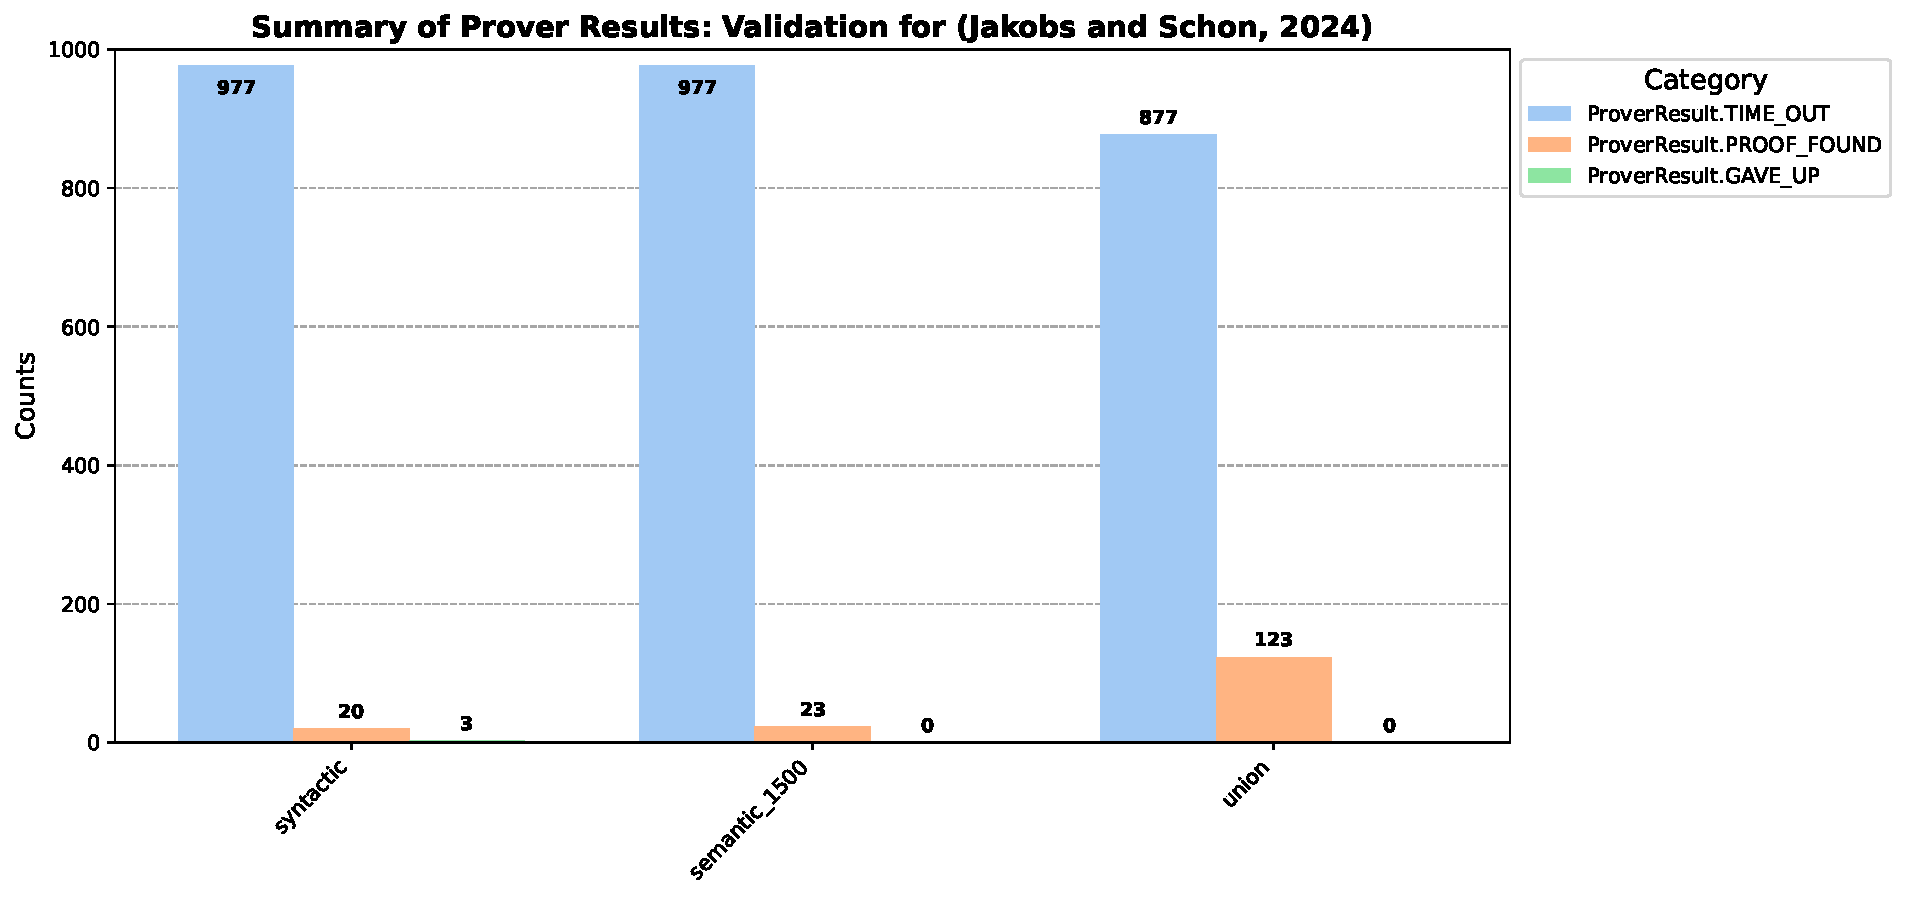
\includegraphics[width=\textwidth]{standard_mode_noAdded_output.pdf}
        \caption{Reengineering of results from \cite{Schon2024}}
        \label{fig:reengineering}
    \end{figure}

    \FloatBarrier

    \item Theorem prover performance is evaluated based on:
    \begin{itemize}
        \item A high percentage of test cases resulted in timeouts or unsuccessful proof attempts, illustrating the difficulty of proving conjectures without additional axioms.
        \item The success rate for proof discovery remained low, suggesting that the standard mode lacks sufficient knowledge for effective inference.
        \item The dataset incorporates multiple axiom selection techniques, including syntactic, semantic-based, and union-based selection.
    \end{itemize}

    \item The distribution of results shows:
    \begin{itemize}
        \item The prover executed 977 test cases, applying each axiom selection approach independently.
        \item The number of successfully proven conjectures was relatively low, reinforcing the importance of improved axiom selection techniques.
        \item Some conjectures had no successful proofs, highlighting weaknesses in current selection strategies.
    \end{itemize}

    \item Implications for further research:
    \begin{itemize}
        \item The findings suggest that semantic similarity alone is insufficient for effective axiom selection.
        \item Further experiments should explore whether the integration of core axioms leads to improved proof success rates.
        \item Analyzing the relationship between axiom complexity and proof success may provide additional insights into theorem proving behavior.
    \end{itemize}
\end{itemize}

\clearpage

\section{Analysis of Reengineering}

The reengineered results are analyzed to better understand proof complexity and selection effectiveness.

\begin{itemize}
    \item The mean variable count in proofs is examined.
    \begin{figure}[h!]
        \centering
        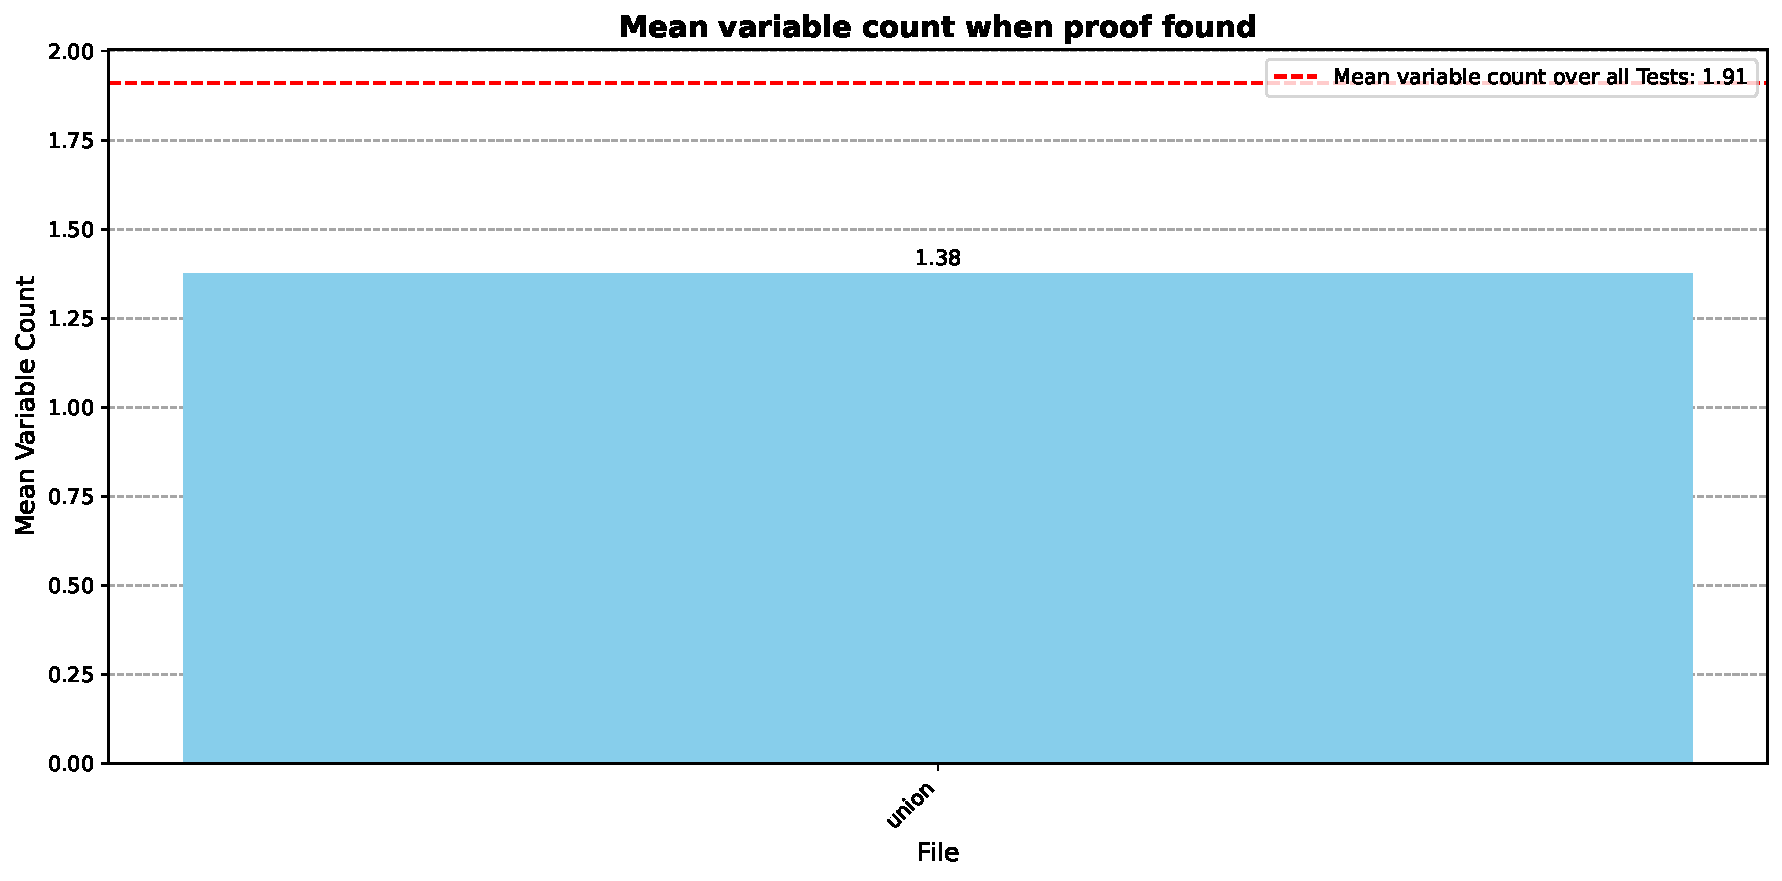
\includegraphics[width=\textwidth]{variable_count_noauto.pdf}
        \caption{Variable count in proofs}
        \label{fig:variable_count}
    \end{figure}
    \FloatBarrier

    \item The count of special symbols in proofs is analyzed.
    \begin{figure}[h!]
        \centering
        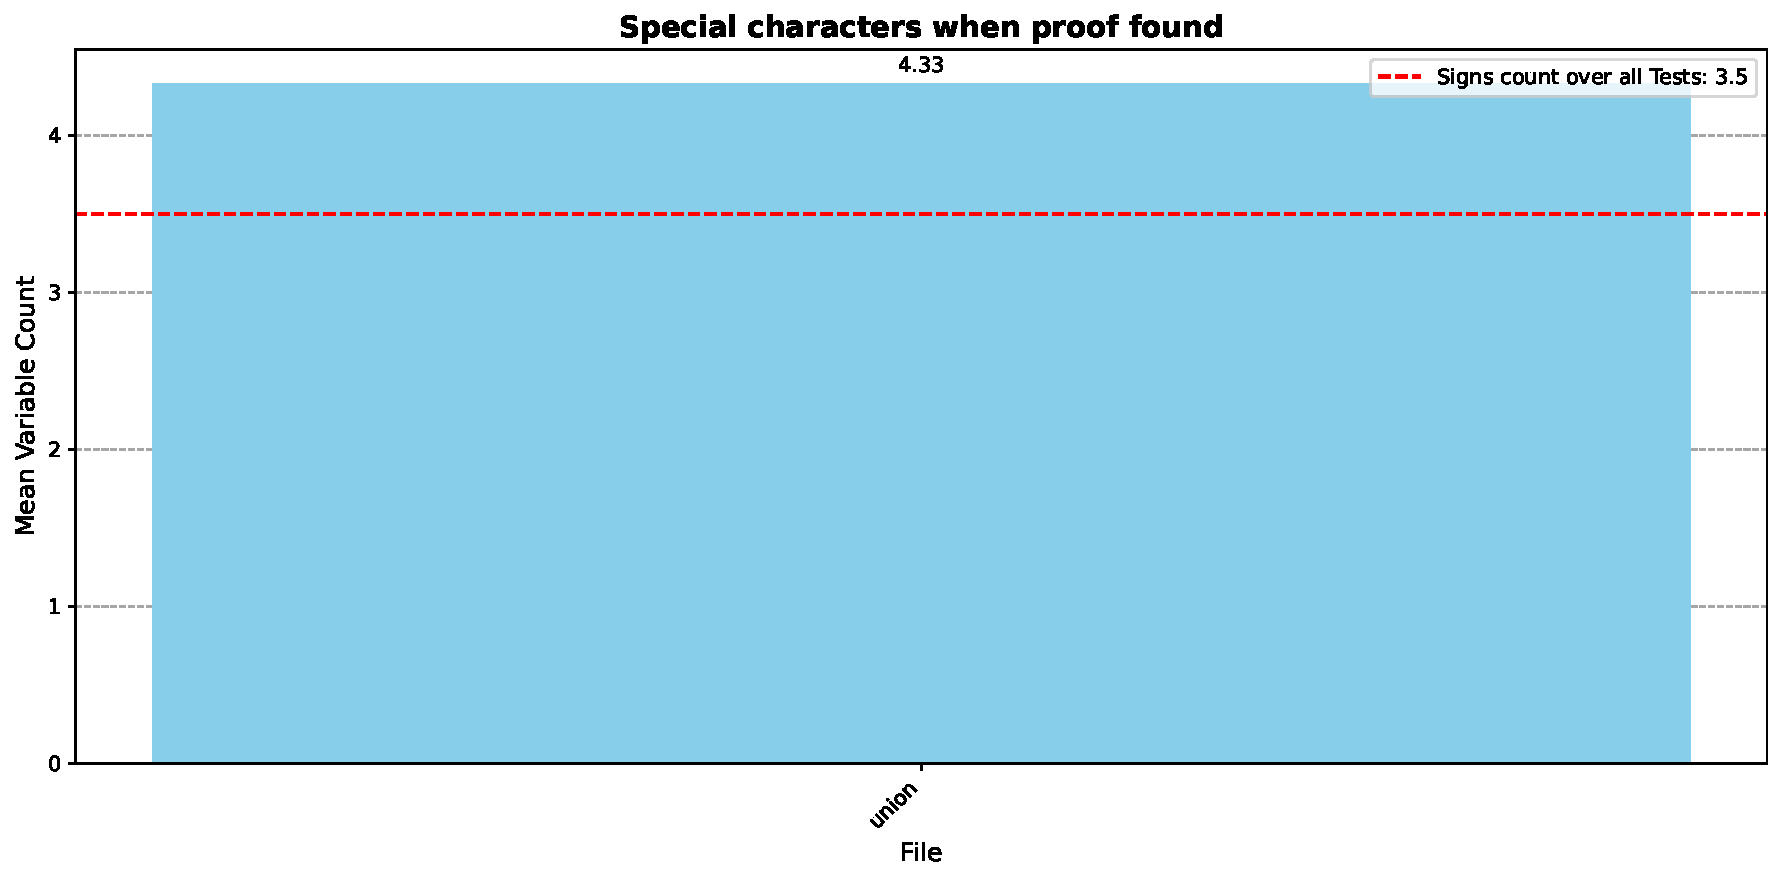
\includegraphics[width=\textwidth]{signs_count_noauto.pdf}
        \caption{Special character count}
        \label{fig:count_signs}
    \end{figure}

    \item The character count across all test cases is examined.
    \begin{figure}[h!]
        \centering
        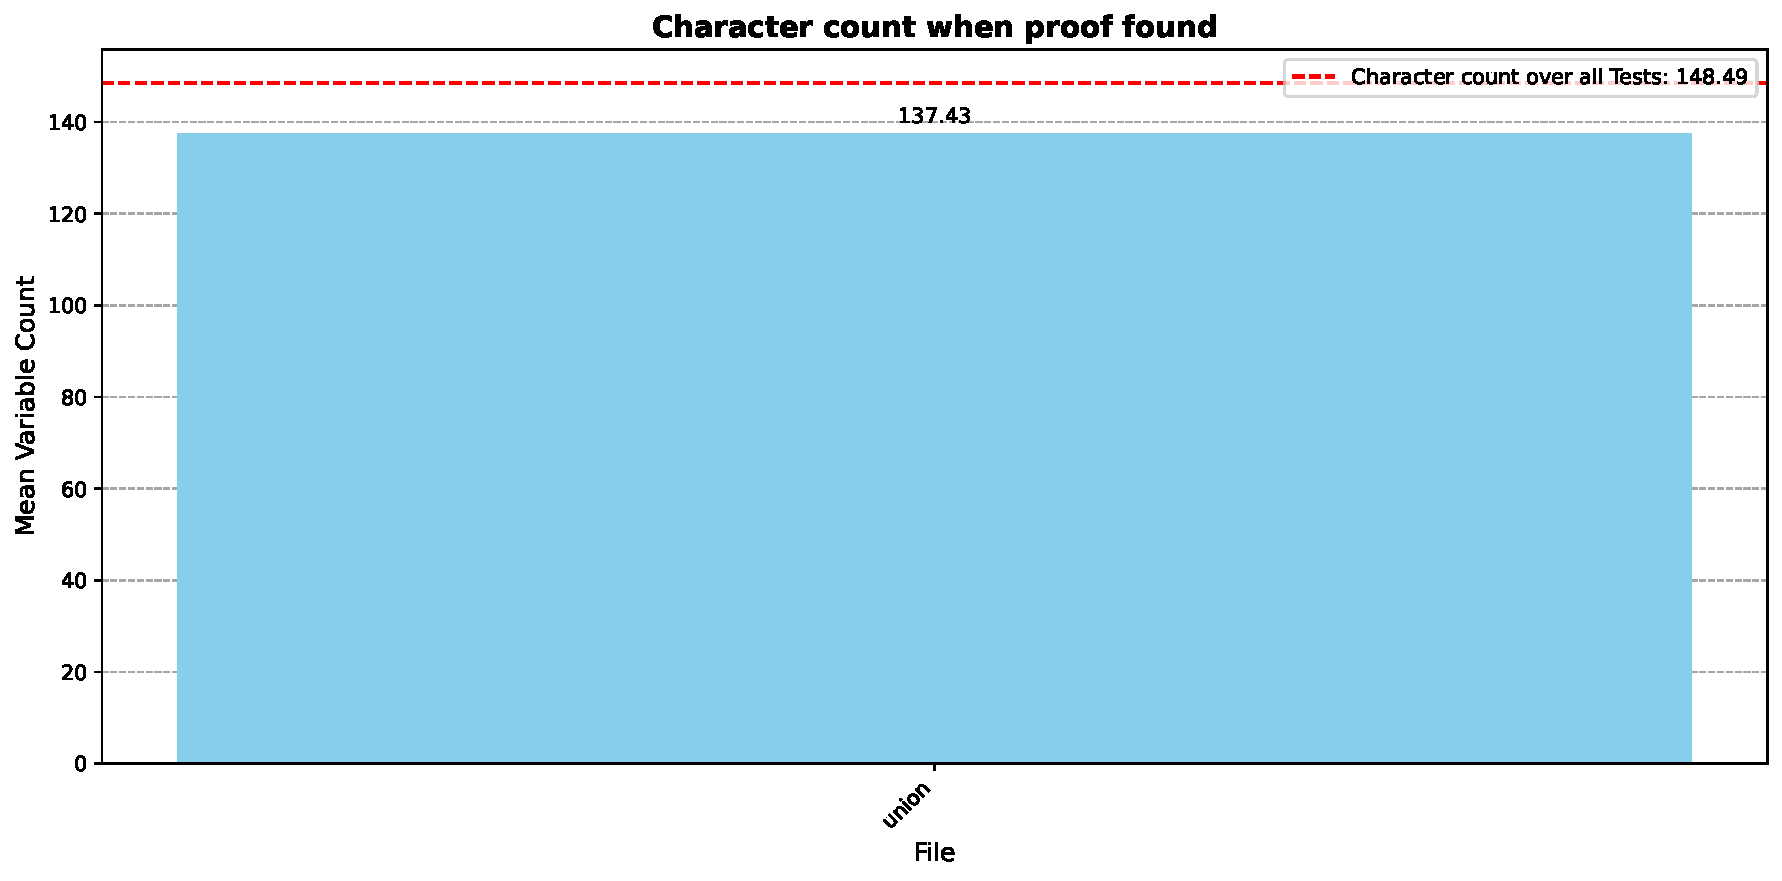
\includegraphics[width=\textwidth]{character_count_noauto.pdf}
        \caption{Character count distribution}
        \label{fig:character_count}
    \end{figure}

    \FloatBarrier

    \item The cosine similarity between axioms and conjectures is analyzed to determine whether similarity influences proof success.
    \begin{figure}[h!]
        \centering
        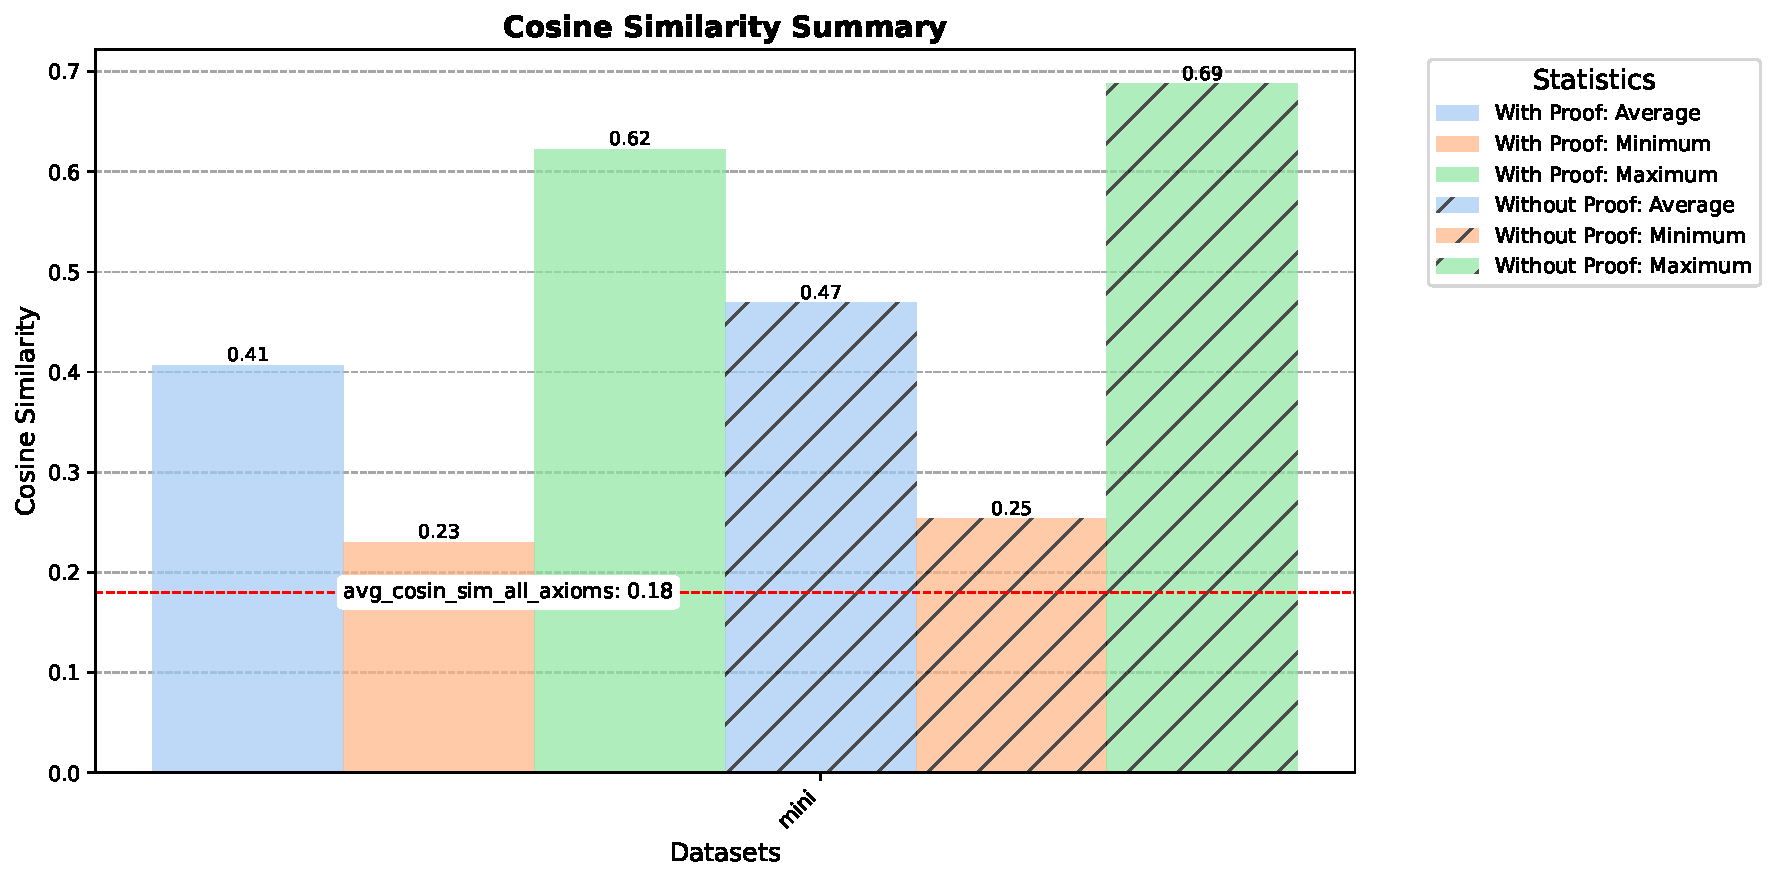
\includegraphics[width=\textwidth]{cosine_similarity_mini_noAdded_summary.pdf}
        \caption{Cosine similarity distribution}
        \label{fig:cosine_similarity}
    \end{figure}
    \FloatBarrier

    The results suggest that provable conjectures often have lower axiom similarity. This indicates that proving a conjecture may require bridging different concepts rather than simply refining closely related axioms.
\end{itemize}

\clearpage

\section{Integration of Core Axioms}

The integration of core axioms into the selection process is evaluated.

\begin{itemize}
    \item The results of theorem proving with core axioms are examined.
    \begin{figure}[h!]
        \centering
        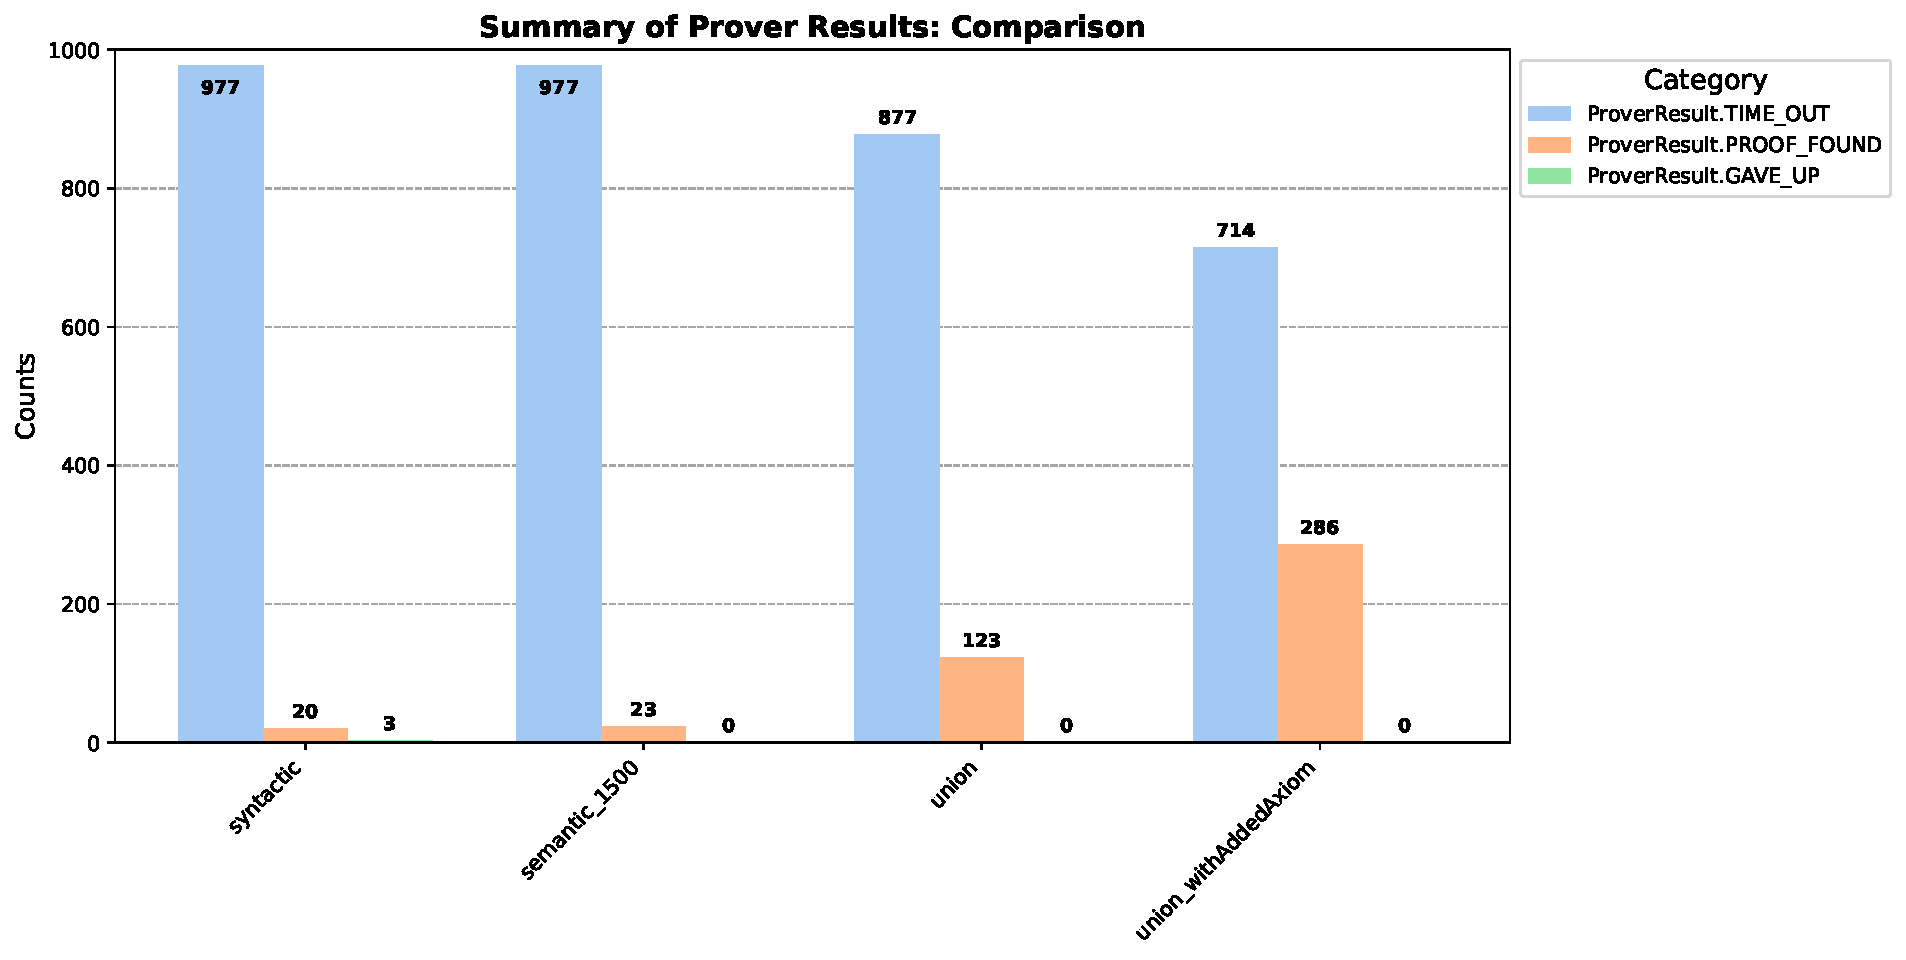
\includegraphics[width=\textwidth]{standard_mode_output.pdf}
        \caption{Summary of prover results with core axioms}
        \label{fig:prover_results_with_core_axioms}
    \end{figure}
    \FloatBarrier

    \item Cosine similarity is compared across different selection methods.
    \begin{figure}[h!]
        \centering
        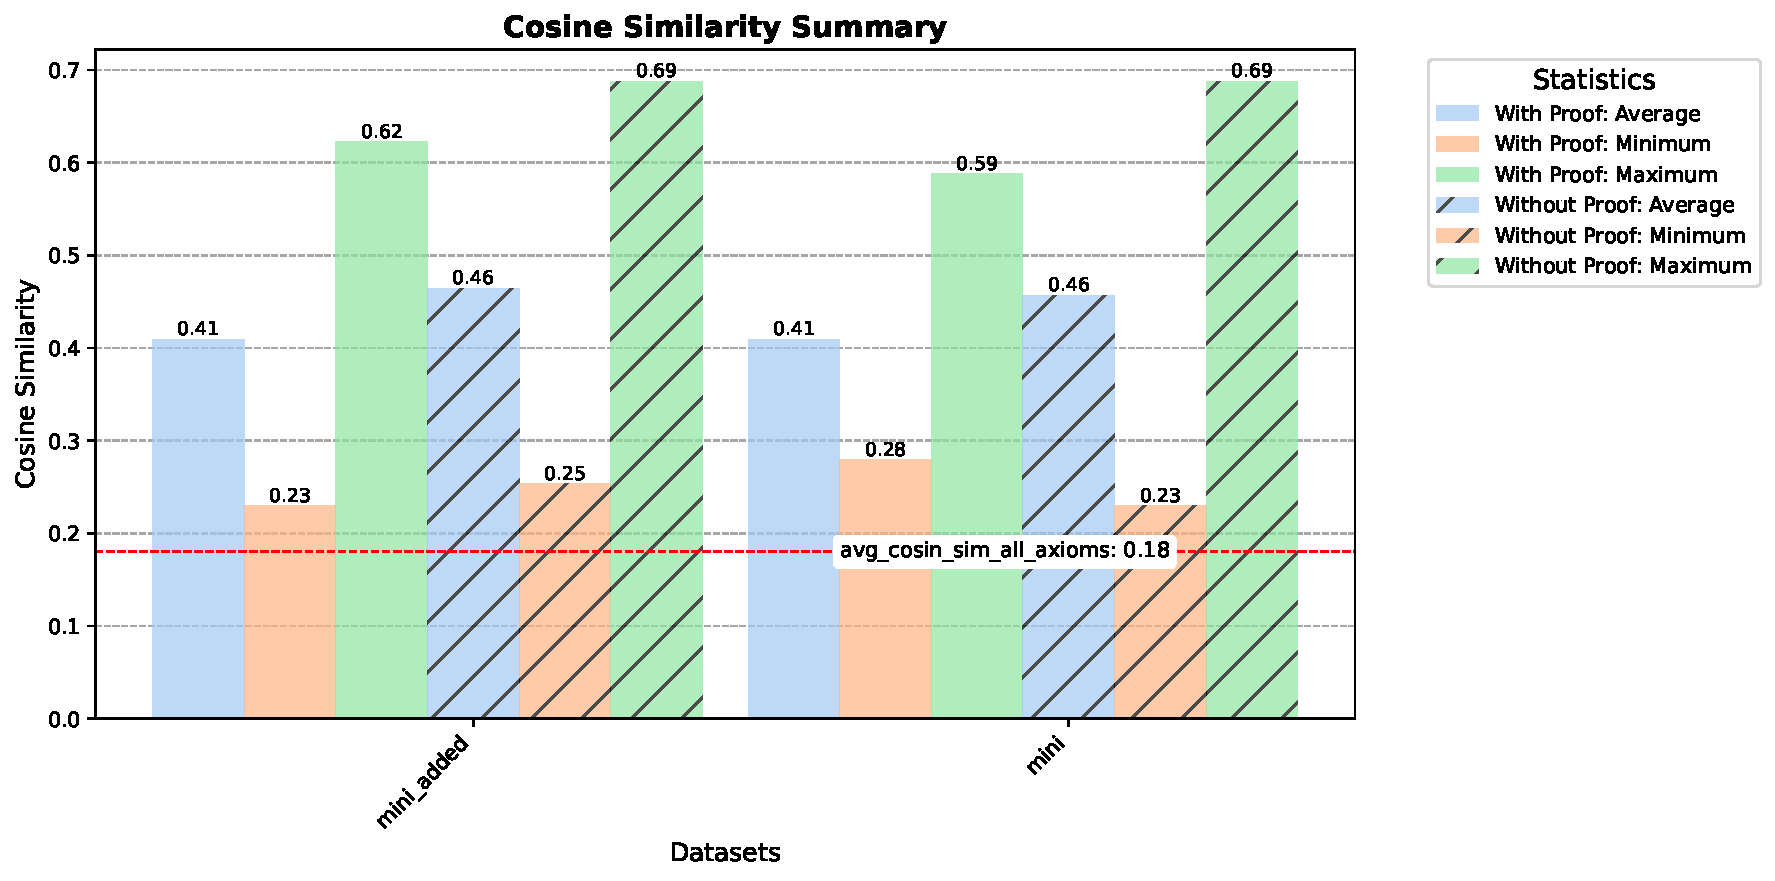
\includegraphics[width=\textwidth]{cosine_similarity_mini_summary.pdf}
        \caption{Cosine similarity comparison}
        \label{fig:prover_results_standard}
    \end{figure}
    \FloatBarrier
\end{itemize}

\clearpage

\section{Comparison of Large Language Models}

The performance of different large language models in axiom selection is assessed.

\begin{itemize}
    \item The results of theorem proving with different models are analyzed.
    \begin{figure}[h!]
        \centering
        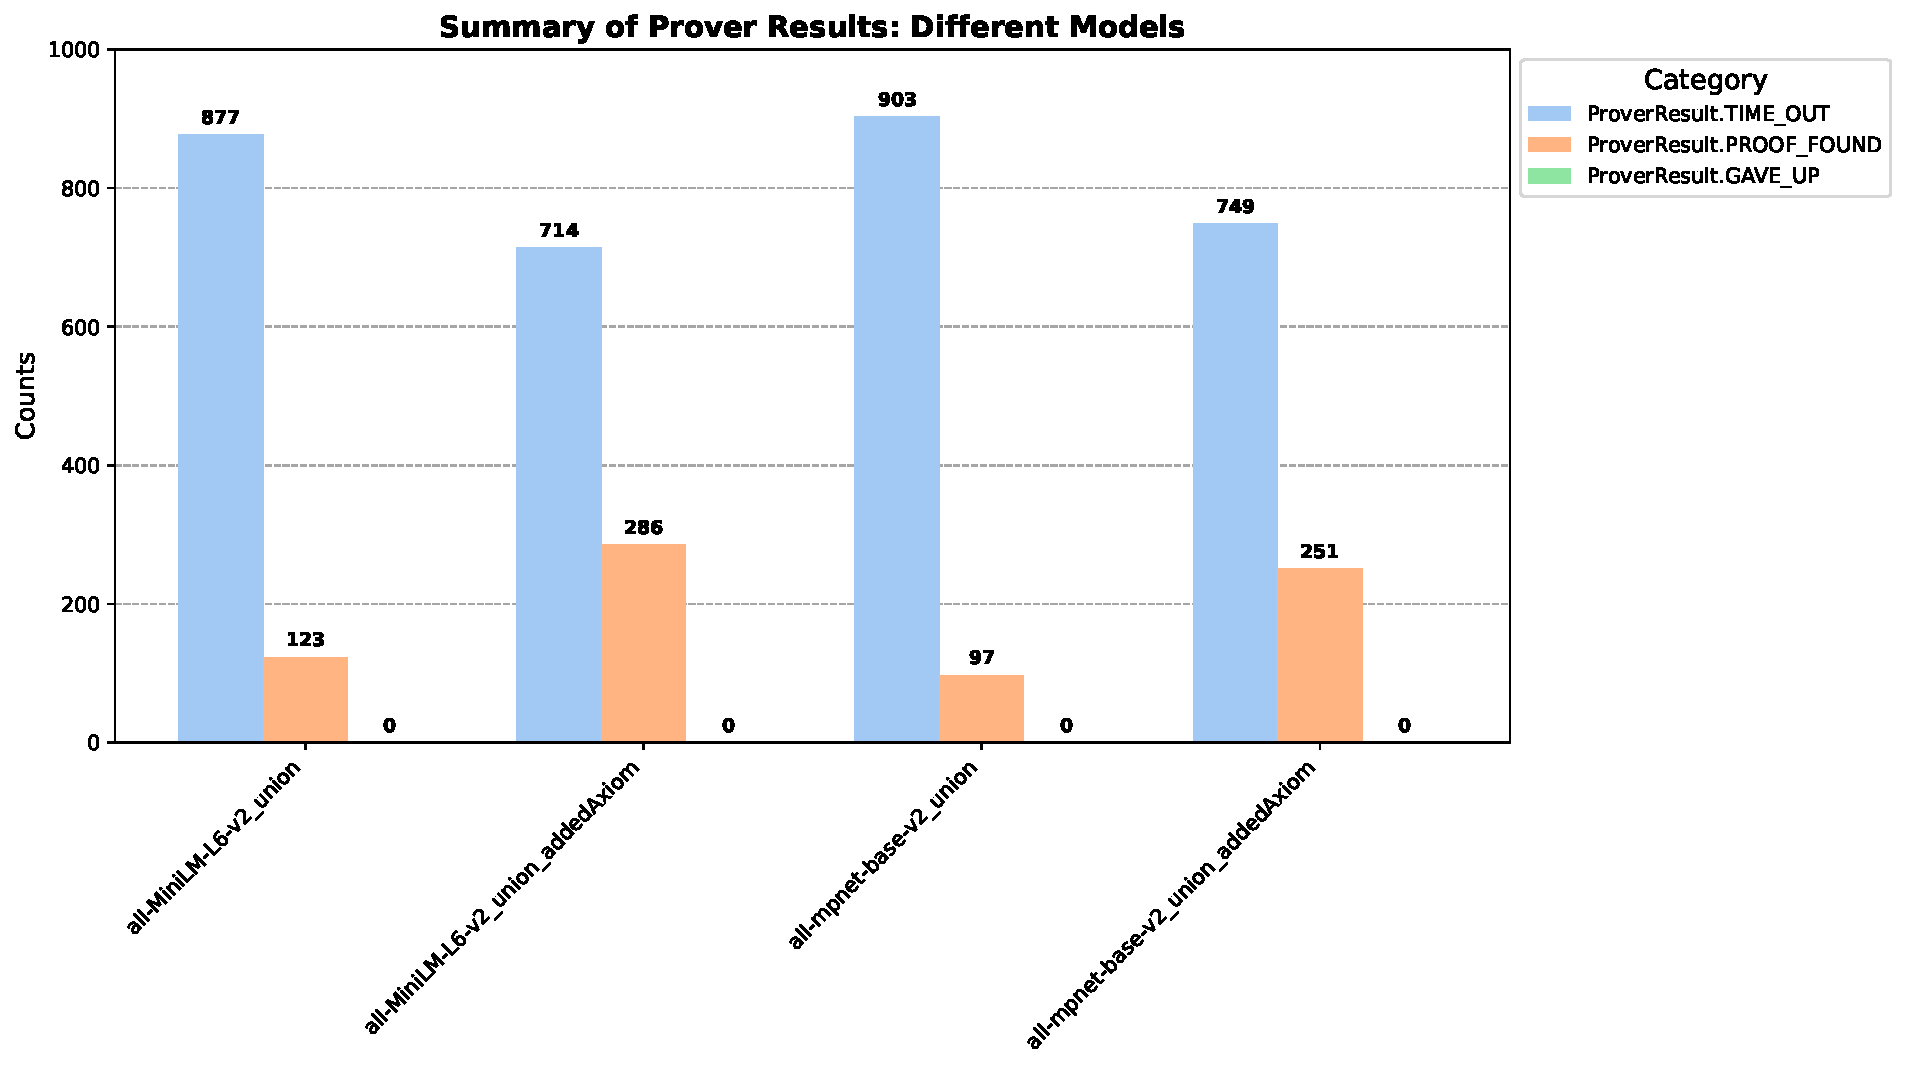
\includegraphics[width=\textwidth]{different_mode_output.pdf}
        \caption{Summary of prover results with different models}
        \label{fig:results_different_models}
    \end{figure}        
    \FloatBarrier

    \item The cosine similarity of selected axioms is compared.
    \begin{figure}[h!]
        \centering
        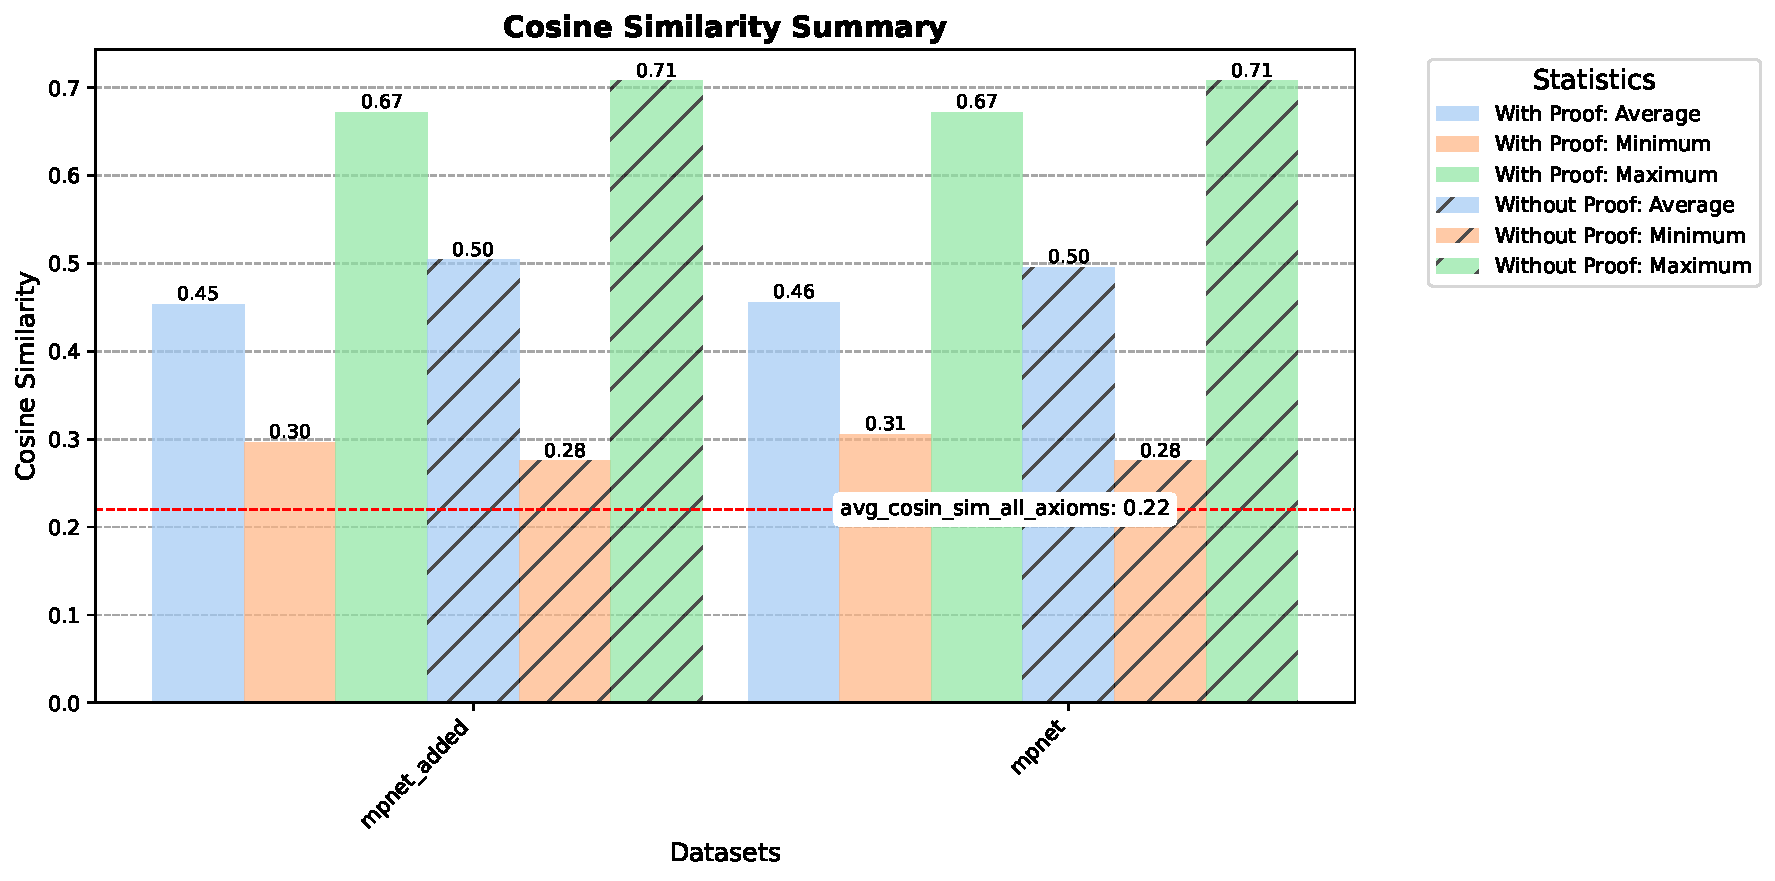
\includegraphics[width=\textwidth]{cosine_similarity_mpnet_summary.pdf}
        \caption{Cosine similarity in different models}
        \label{fig:cosine_similarity_mpnet}
    \end{figure}
    \FloatBarrier
\end{itemize}

\clearpage

\section{Evaluation of Theorem Prover Configurations}

The effect of different theorem prover configurations is analyzed.

\begin{itemize}
    \item The performance of Satauto mode is examined.
    \begin{figure}[h!]
        \centering
        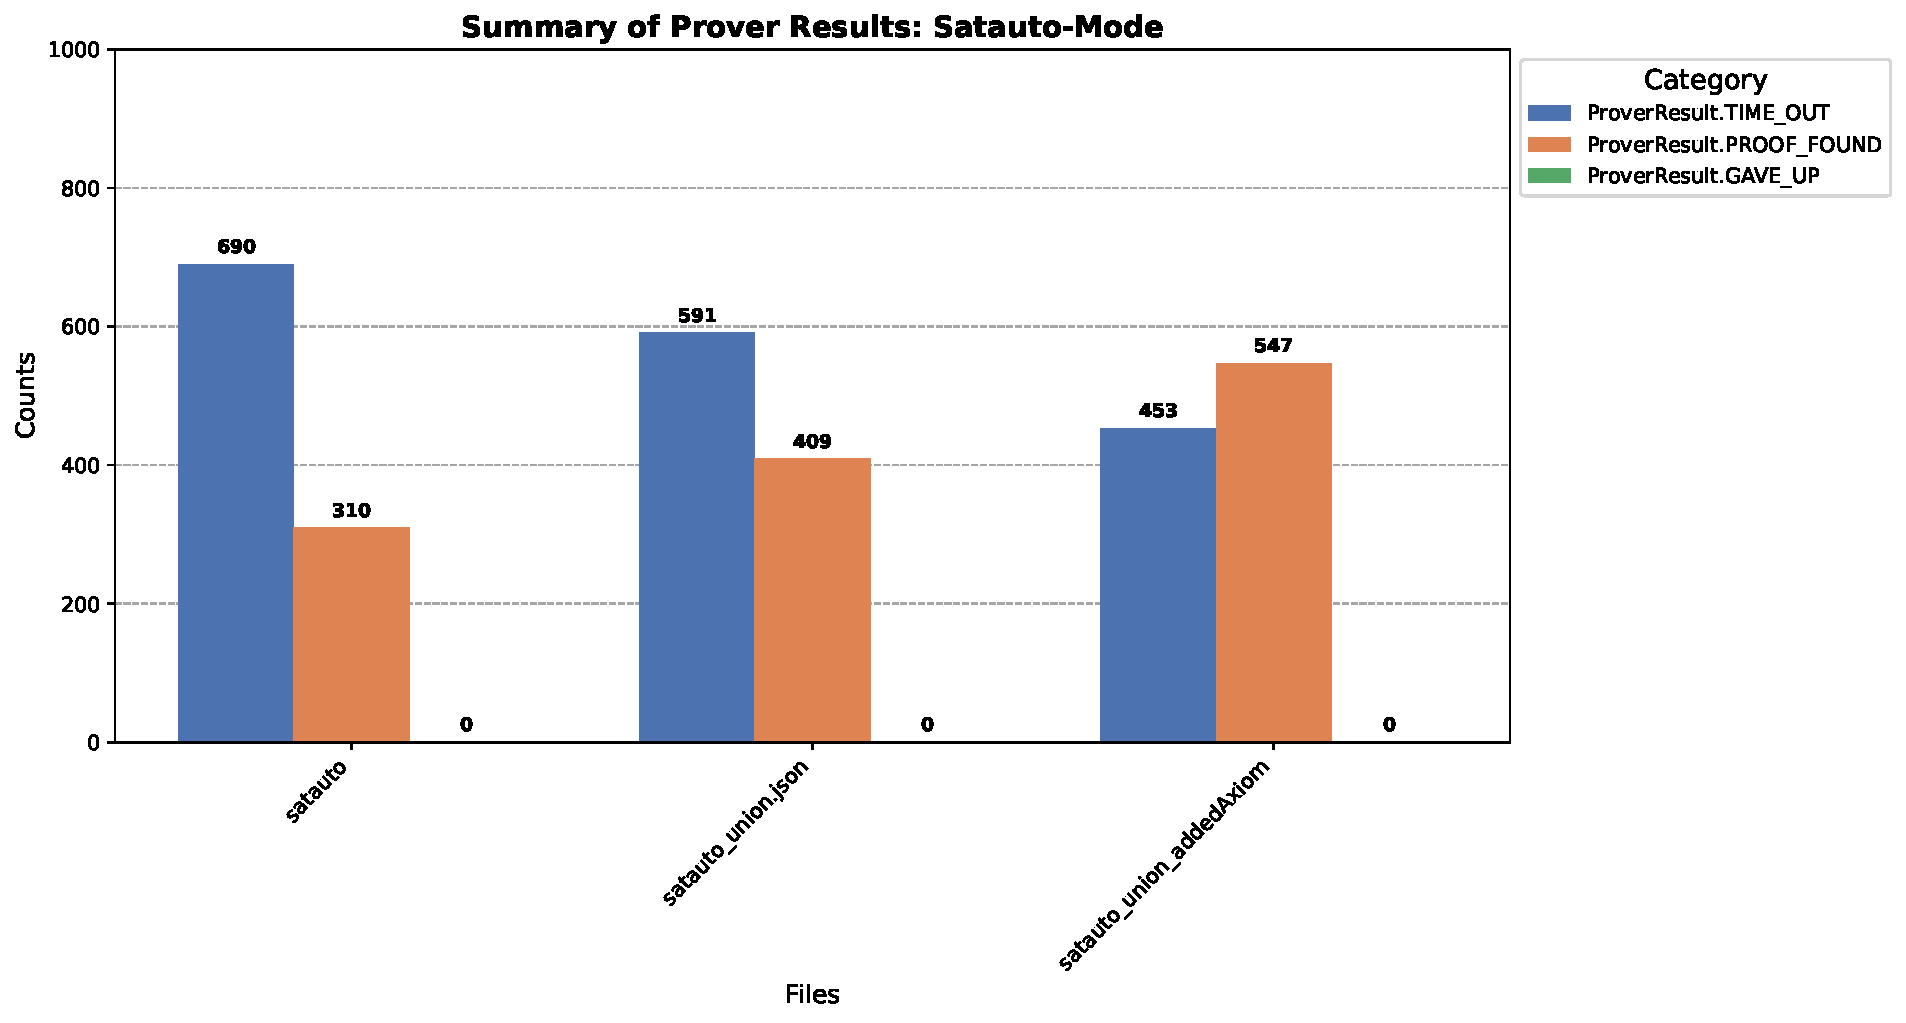
\includegraphics[width=\textwidth]{satauto_mode_output.pdf}
        \caption{Summary of prover results in Satauto mode}
        \label{fig:prover_results_satauto}
    \end{figure}
    \FloatBarrier

    \item The effect of auto mode, which uses SInE and search heuristics, is assessed.
    \begin{figure}[h!]
        \centering
        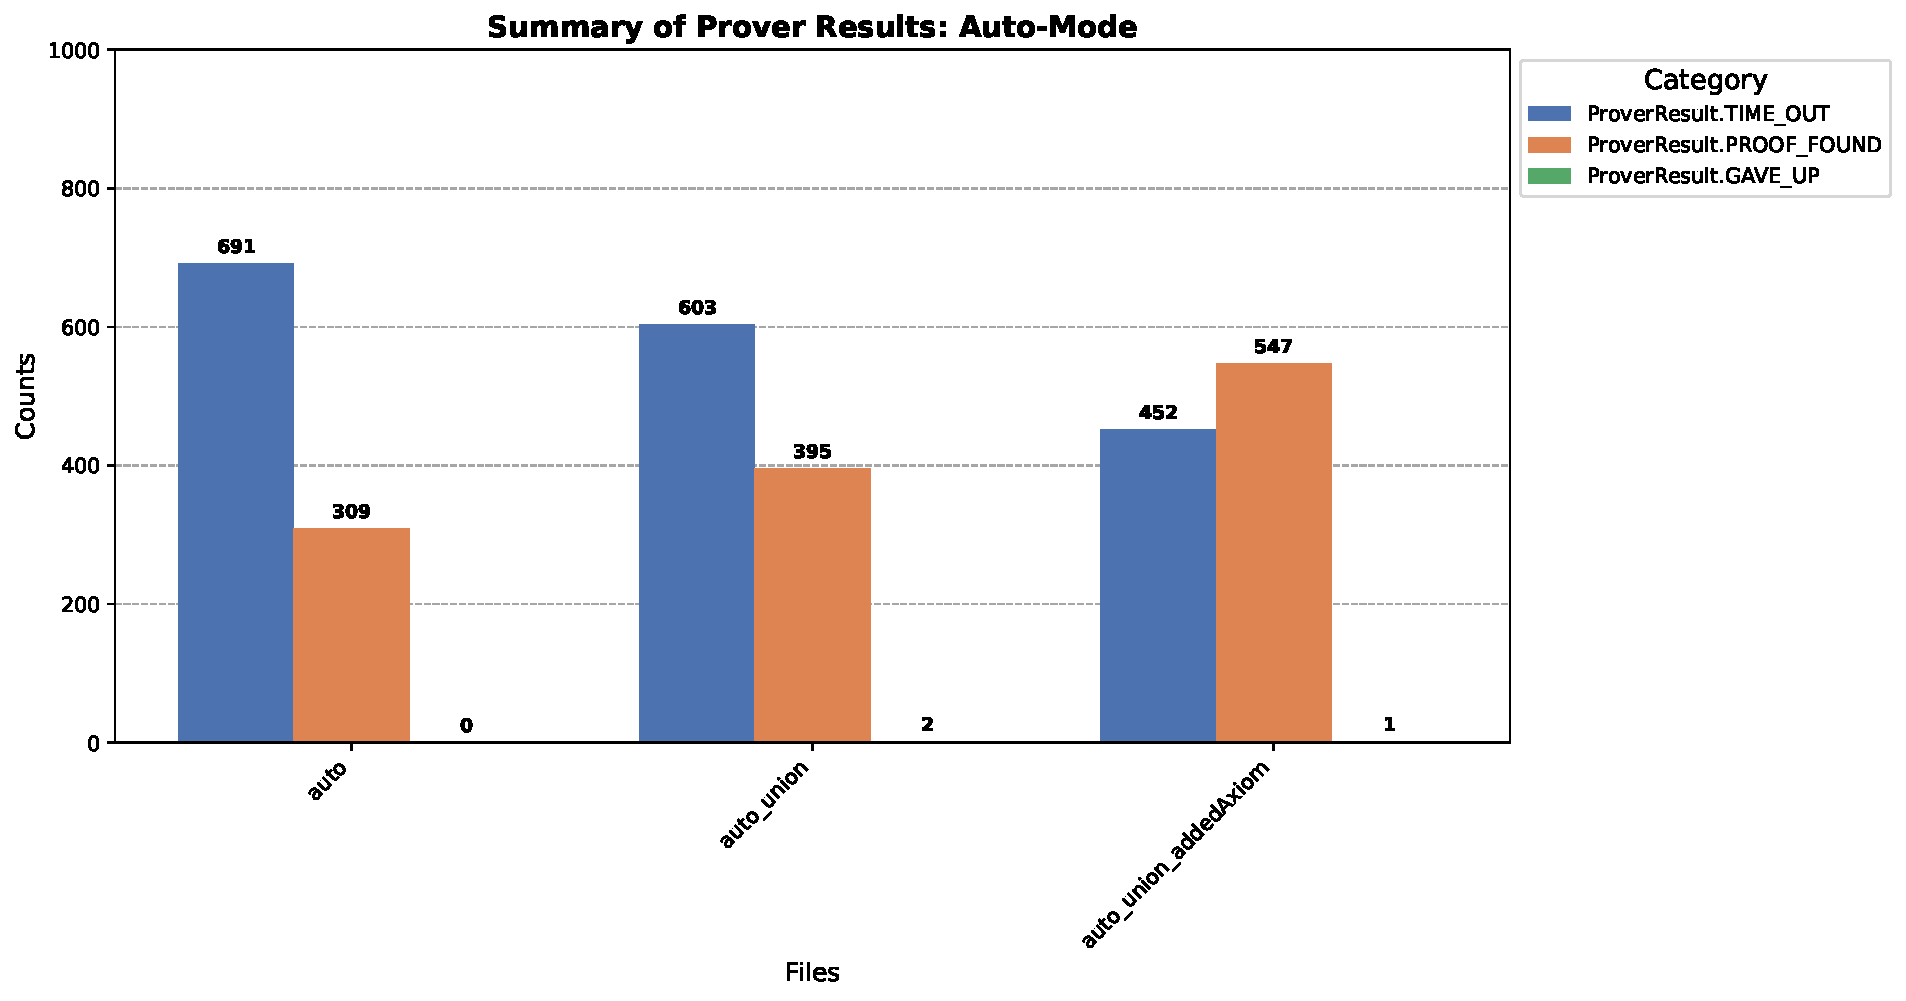
\includegraphics[width=\textwidth]{auto_mode_output.pdf}
        \caption{Summary of prover results in Auto mode}
        \label{fig:prover_results_auto}
    \end{figure}
    \FloatBarrier
\end{itemize}

\clearpage


\chapter{Conclusion}
\label{chapter-conclusion}
Conclusion.
\clearpage

\chapter{Future work}
\label{chapter-futerwork}

Future work.




% Normally, the bibliography comes next at this point. Do *not* (try
% to) include further indices and tables like an index or
% a list of figures or a list of tables or such things. Nobody
% actually uses them and they just use up space. 
%
% You *can* however include a glossary, if this seems appropriate. It
% goes here as an unnumbered chapter. Most thesis will *not* need a
% glossary: a well-written text (re)explains strange words and
% concepts as necessary. However, there are situations where a
% glossary may be helpful.

%%%
% 
% Bibliographies
%
%%%
%
% The uzl-thesis class will load biblatex for the bibliography
% management. This is a powerful package, see its documentation for
% details. The styles will be setup correctly and automatically by
% choosing one of the two style keys as described earlier.
%
% In order for the bibliography to work, run latex in the following
% order (which is the standard order):
% 
% > lualatex thesis-example
% > bibtex thesis-example
% > lualatex thesis-example
% 
% Add BibTeX files using \addbibresource or use the {bibtex entries}
% environment (see below).
%
%%%
%
% Although everyting is normally setup automatically, you can change
% the options passed to biblatex using the key 'biblatex';
% for instance,
%
%   \UzLThesisSetup{biblatex={firstinits=false}}
%
% will switch off shortened first names. Normally, you will not need
% this key in your preamble. 
% 
% Note that the bibtex program is used as the 'backend' of biblatex
% by default (rather than biber, which is the preferred program of
% biblatex). This means that you can (and must) run *bibtex* after you
% have run lualatex on your thesis. If you wish to use biber instead
% of bibtex, say 'biblatex={backend=biber}'. 
% 
%%%
%
% The following environment is optional. It allows you to keep the
% bibtex entries for your thesis right here in the thesis file. What
% happens is that each time this tex file is processed, the contents
% of the following environment gets written to the file
% \jobname-bibtex-entries.bib (this file gets overwritten each
% time). Independently, \addbibresource{\jobname-bibtex-entries.bib}
% is always called if the file \jobname-bibtex-entries.bib
% exists. 
%
% In result, you can edit and keep the bibliography's bibtex entries
% right here. If you change something here, run latex, then bibtex,
% then latex once more.
%
% If you would like to manage the bibtex entries in a separate file,
% remove the below environment, delete the \jobname-bibtex-entries.bib
% file and instead write
%
% \addbibresource{filename-of-your-bibtex-file.bib}
%
% in the preamble.
%
%%%


% !!!!!!!!!!!!!!!!!!!!!!!!!!!!!!!!!!
% !!! Your action is needed here !!!
% !!!!!!!!!!!!!!!!!!!!!!!!!!!!!!!!!!
%
% Replace following example entries with the ones of your thesis.

\begin{bibtex-entries}
@inproceedings{Schon2024,
    author={Jakobs, Oliver and Schon, Claudia},
    editor={Hotho, Andreas and Rudolph, Sebastian},
    title={Context-Specific Selection of Commonsense Knowledge Using Large Language Models},
    booktitle={KI 2024: Advances in Artificial Intelligence},
    year={2024},
    publisher={Springer Nature Switzerland},
    address={Cham},
    pages={218--231},
    abstract={In the field of automated reasoning, practical applications often face a significant challenge: knowledge bases are typically too large to be fully processed by theorem provers. To still be able to prove that a given goal follows from a large knowledge base, selection techniques are used to determine the parts of the knowledge base that are relevant to the goal. Traditional selection techniques used for this task are usually syntax-based and often overlook a crucial aspect---the meaning of symbol names and axioms. Especially in commonsense reasoning scenarios, the meaning embedded in the symbol names provides invaluable insights. For example, in a proof task using the symbol name cow, it intuitively makes more sense to select formulae using the symbol name calf than formulae using the symbol name weapon. To address this gap, our paper introduces a selection technique that exploits the capabilities of large language models. This technique focuses on contextually related formulae, closely aligning the selected part of the knowledge base with the context of the goal. The approach is implemented and we present a series of experiments that show promising results.},
    isbn={978-3-031-70893-0}
}

@article{Àlvez2014,
    author = {Àlvez, Javier and Lucio, Paqui and Rigau, German},
    year = {2014},
    month = {10},
    pages = {80-116},
    title = {Adimen-SUMO: Reengineering an Ontology for First-Order Reasoning},
    volume = {8},
    journal = {International Journal on Semantic Web and Information Systems},
    doi = {10.4018/jswis.2012100105}
}

@inproceedings{Hoder2011,
    author={Hoder, Kry{\v{s}}tof and Voronkov, Andrei},
    editor={Bj{\o}rner, Nikolaj and Sofronie-Stokkermans, Viorica},
    title={Sine Qua Non for Large Theory Reasoning},
    booktitle={Automated Deduction -- CADE-23},
    year={2011},
    publisher={Springer Berlin Heidelberg},
    address={Berlin, Heidelberg},
    pages={299--314"},
    abstract={One possible way to deal with large theories is to have a good selection method for relevant axioms. This is confirmed by the fact that the largest available first-order knowledge base (the Open CYC) contains over 3 million axioms, while answering queries to it usually requires not more than a few dozen axioms. A method for axiom selection has been proposed by the first author in the Sumo INference Engine (SInE) system. SInE has won the large theory division of CASC in 2008. The method turned out to be so successful that the next two years it was used by the winner as well as by several other competing systems. This paper contains the presentation of the method and describes experiments with it in the theorem prover Vampire.},
    isbn={978-3-642-22438-6}
}

@inproceedings{Roederer2009,
    author={Roederer, Alex and Puzis, Yury and Sutcliffe, Geoff},
    editor={Schmidt, Renate A.},
    title={Divvy: An ATP Meta-system Based on Axiom Relevance Ordering},
    booktitle={Automated Deduction -- CADE-22},
    year={2009},
    publisher={Springer Berlin Heidelberg},
    address={Berlin, Heidelberg},
    pages={157--162"}
    abstract={This paper describes two syntactic relevance orderings on the axioms available for proving a given conjecture, and an ATP meta-system that uses the orderings to select axioms to use in proof attempts. The system has been evaluated, and the results show that it is effective.},
    isbn={978-3-642-02959-2}
}

@inproceedings{Sutcliffe2007,
    author={Sutcliffe, Geoff and Puzis, Yury},
    editor={Pfenning, Frank},
    title={SRASS - A Semantic Relevance Axiom Selection System},
    booktitle={Automated Deduction -- CADE-21},
    year={2007},
    publisher={Springer Berlin Heidelberg},
    address={Berlin, Heidelberg},
    pages={295--310},
    abstract={This paper describes the design, implementation, and testing of a system for selecting necessary axioms from a large set also containing superfluous axioms, to obtain a proof of a conjecture. The selection is determined by semantics of the axioms and conjecture, ordered heuristically by a syntactic relevance measure. The system is able to solve many problems that cannot be solved alone by the underlying conventional automated reasoning system.},
    isbn={978-3-540-73595-3}
}

@article{Álvez2017,
    author = {Álvez, Javier and Hermo, Montserrat and Lucio, Paqui and Rigau, German},
    year = {2017},
    month = {05},
    pages = {},
    title = {Automatic White-Box Testing of First-Order Logic Ontologies},
    volume = {29},
    journal = {Journal of Logic and Computation},
    doi = {10.1093/logcom/exz001}
}


@inproceedings{Schulz2019,
  author    = {Stephan Schulz and Simon Cruanes and Petar Vukmirovi{\'c}},
  title     = {Faster, Higher, Stronger: {E} 2.3},
  booktitle = {Proceedings of the 27th International Conference on Automated Deduction (CADE-27)},
  editor    = {Pascal Fontaine},
  year      = {2019},
  number    = {11716},
  series    = {Lecture Notes in Artificial Intelligence (LNAI)},
  pages     = {495--507},
  publisher = {Springer}
}


@article{Miller1991,
  author    = {George A. Miller and Walter G. Charles},
  title     = {Contextual Correlates of Semantic Similarity},
  journal   = {Language and Cognitive Processes},
  volume    = {6},
  number    = {1},
  pages     = {1--28},
  year      = {1991},
  publisher = {Routledge},
  doi       = {10.1080/01690969108406936},
  url       = {https://doi.org/10.1080/01690969108406936},
  eprint    = {https://doi.org/10.1080/01690969108406936}
}


@InProceedings{Schon2023,
  author    = {Claudia Schon},
  editor    = {Dietmar Seipel and Alexander Steen},
  title     = {Associative Reasoning for Commonsense Knowledge},
  booktitle = {KI 2023: Advances in Artificial Intelligence},
  year      = {2023},
  publisher = {Springer Nature Switzerland},
  address   = {Cham},
  pages     = {170--183},
  isbn      = {978-3-031-42608-7}
}


@inproceedings{Kiros2015SkipThought,
  author    = {Ryan Kiros and Yukun Zhu and Ruslan Salakhutdinov and Richard S. Zemel and Raquel Urtasun and Antonio Torralba and Sanja Fidler},
  title     = {Skip-Thought Vectors},
  booktitle = {Advances in Neural Information Processing Systems 28: Annual Conference on Neural Information Processing Systems 2015 (NeurIPS)},
  editor    = {Corinna Cortes and Neil D. Lawrence and Daniel D. Lee and Masashi Sugiyama and Roman Garnett},
  pages     = {3294--3302},
  year      = {2015},
  address   = {Montreal, Quebec, Canada},
  month     = {December 7-12}
}

@inproceedings{Furbach2019WordEmbeddings,
  author    = {Ulrich Furbach and Teresa Kr{\"a}mer and Claudia Schon},
  editor    = {Pascal Fontaine},
  title     = {Names Are Not Just Sound and Smoke: Word Embeddings for Axiom Selection},
  booktitle = {Automated Deduction -- CADE 27},
  year      = {2019},
  publisher = {Springer International Publishing},
  address   = {Cham},
  pages     = {250--268},
  abstract  = {First-order theorem proving with large knowledge bases makes it necessary to select those parts of the knowledge base, that are necessary to prove the theorem at hand. We extend syntactic axiom selection procedures like SInE to use semantics of symbol names. For this, not only occurrences of symbol names but also semantically similar names are taken into account. We use a similarity measure based on word embeddings. An evaluation of this similarity based SInE is given using problems from TPTP's CSR problem class and Adimen-SUMO. This evaluation is done with two very different systems, namely the Hyper tableau prover and the saturation based system E.},
  isbn      = {978-3-030-29436-6},
  doi       = {10.1007/978-3-030-29436-6_15}
}

@inproceedings{Bayerkuhnlein2023,
  author    = {Moritz Bayerkuhnlein},
  title     = {SUMO Wrestling Winograd Schemas},
  booktitle = {Proceedings of a University Research Project},
  year      = {2023},
  institution = {University of Bamberg},
  address   = {Bamberg, Germany},
  url       = {https://www.uni-bamberg.de}
}

@incollection{Johnson-Laird1989,
  author    = {P. N. Johnson-Laird},
  title     = {Mental Models},
  booktitle = {Foundations of Cognitive Science},
  editor    = {M. I. Posner},
  pages     = {469--499},
  publisher = {The MIT Press},
  year      = {1989}
}

@inproceedings{Levesque2012,
  author    = {Hector Levesque and Ernest Davis and Leora Morgenstern},
  title     = {The Winograd Schema Challenge},
  booktitle = {Thirteenth International Conference on the Principles of Knowledge Representation and Reasoning},
  year      = {2012}
}

@inproceedings{Mikolov2013,
  author    = {Tom{\'a}s Mikolov and Kai Chen and Greg Corrado and Jeffrey Dean},
  title     = {Distributed Representations of Words and Phrases and Their Compositionality},
  booktitle = {Advances in Neural Information Processing Systems 26 (NeurIPS)},
  editor    = {Christopher J. C. Burges and Leon Bottou and Max Welling and Zoubin Ghahramani and Kilian Q. Weinberger},
  year      = {2013},
  pages     = {3111--3119},
  url       = {https://proceedings.neurips.cc/paper/2013/hash/9aa42b31882ec039965f3c4923ce901b-Abstract.html}
}

@article{Bojanowski2017,
  author    = {Piotr Bojanowski and Edouard Grave and Armand Joulin and Tomas Mikolov},
  title     = {Enriching Word Vectors with Subword Information},
  journal   = {Transactions of the Association for Computational Linguistics},
  volume    = {5},
  year      = {2017},
  pages     = {135--146},
  doi       = {10.1162/TACL_A_00051},
  url       = {https://doi.org/10.1162/tacl_a_00051}
}

@inproceedings{Pennington2014,
  author    = {Jeffrey Pennington and Richard Socher and Christopher Manning},
  title     = {GloVe: Global Vectors for Word Representation},
  booktitle = {Proceedings of the 2014 Conference on Empirical Methods in Natural Language Processing (EMNLP)},
  editor    = {Alessandro Moschitti and Bo Pang and Walter Daelemans},
  year      = {2014},
  address   = {Doha, Qatar},
  publisher = {Association for Computational Linguistics},
  pages     = {1532--1543},
  doi       = {10.3115/v1/D14-1162},
  url       = {https://aclanthology.org/D14-1162}
}

@inproceedings{Devlin2019,
  author    = {Jacob Devlin and Ming{-}Wei Chang and Kenton Lee and Kristina Toutanova},
  title     = {BERT: Pre-training of Deep Bidirectional Transformers for Language Understanding},
  booktitle = {Proceedings of the 2019 Conference of the North American Chapter of the Association for Computational Linguistics: Human Language Technologies, {NAACL-HLT} 2019},
  pages     = {4171--4186},
  year      = {2019},
  publisher = {Association for Computational Linguistics},
  doi       = {10.18653/v1/N19-1423},
  url       = {https://aclanthology.org/N19-1423/}
}

@inproceedings{Niles2001,
  author    = {Ian Niles and Adam Pease},
  title     = {Towards a Standard Upper Ontology},
  booktitle = {Proceedings of the International Conference on Formal Ontology in Information Systems ({FOIS} 2001)},
  pages     = {2--9},
  year      = {2001},
  publisher = {ACM},
  doi       = {10.1145/505168.505170},
  url       = {https://doi.org/10.1145/505168.505170}
}






\end{bibtex-entries}


% If you need to have an appendix (I advise against it), insert it
% here using, first, \appendix and then \chapter and then,
% possibly, \section. 
%
% \appendix

\end{document}
